% SN2018.tex
% Darja Maljceva, Vladimir Batagelj
% Analysis of the social networks literature
% ----------------------------------------------------------------------------
% version 0: March 2017
% ----------------------------------------------------------------------------
% https://github.com/bavla/SocNet
% C:\Users\batagelj\work\Python\WoS\SocNet\2018
% ----------------------------------------------------------------------------
%\documentclass[hyperref={pdfstartview={FitBH -32768},
%                         pdfpagemode=FullScreen,
%                         plainpages=false,
%                         colorlinks=true}
%              ]{article}
\documentclass[a4paper,11pt]{article}
\usepackage[english]{babel}
\usepackage{hyperref}
%\usepackage[cp1250]{inputenc}
%\usepackage[utf8]{inputenc}
\usepackage{latexsym}
\usepackage{amsfonts}
\usepackage{times}
\usepackage{xcolor}
\usepackage{graphicx}
\usepackage{crayola}
%\usepackage{datum}
\usepackage{xspace}
\usepackage{algorithmicx}
\usepackage{natbib}
\usepackage{authblk}


\renewcommand{\textfraction}{.05}
\renewcommand{\topfraction}{.95}

\oddsidemargin 5pt \evensidemargin 5pt \marginparwidth 20pt
\marginparsep 10pt \topmargin -12 true mm \headheight 12pt \headsep 25pt
\textheight 23 true cm \textwidth 16 true cm
\columnsep 10pt \columnseprule 0pt

% title page --------------------------------------------------------------

\newcommand*{\affaddr}[1]{#1} % No op here. Customize it for different styles.
\newcommand*{\affmark}[1][*]{\textsuperscript{#1}}
\newcommand*{\email}[1]{\texttt{#1}}

\title{\LARGE\textbf{Social Network Analysis}\protect\\ The evolution of the field}
%\thanks{\textcolor{BrickRed}{\textbf{Applied Statistics}}, Ribno, 23-26. September 2018}

\author{%
Darja Maltseva\affmark[1], Vladimir Batagelj\affmark[1,2,3]\\
\affaddr{\affmark[1]NRU HSE Moscow}\\
\affaddr{\affmark[2]IMFM Ljubljana}\\
\affaddr{\affmark[3]IAM UP Koper}\\
\email{vladimir.batagelj@fmf.uni-lj.si}\\ \email{d.maltseva@gmail.com} %\\
%\affaddr{\LaTeX\ University}%
}
% \author{Darja Maljceva, Vladimir Batagelj  IMFM Ljubljana, IAM UP Koper, NRU HSE Moscow}


% user's macros ----------------------------------------------------------
\newcommand{\Pajek}{\texttt{\textbf{Pajek}}\xspace}
\newcommand{\WoSPajek}{\texttt{\textbf{WoS2Pajek}}\xspace}
%\newcommand{\Pajek}{Pajek}
\newcommand{\keyw}[1]{\textcolor{red}{\emph{#1}}}
\newcommand{\important}[1]{\textcolor{NavyBlue}{#1}}
\newcommand{\RR}{\Bbb{R}}
\newcommand{\NN}{\Bbb{N}}
\newcommand{\ZZ}{\Bbb{Z}}
\newcommand{\QQ}{\Bbb{Q}}
\newcommand{\network}[1]{\mathcal{#1}}
\newcommand{\vertices}[1]{\mathcal{#1}}
\newcommand{\edges}[1]{\mathcal{#1}}
\newcommand{\arcs}[1]{\mathcal{#1}}
\newcommand{\Net}{\network{N}}
\newcommand{\argmin}{\mathop{\mbox{argmin}}\nolimits}
\newcommand{\relation}[1]{\textbf{\emph{$\_\!\_$~#1~$\_\!\_$\,}}}
\newcommand{\functions}[1]{\mathcal{#1}}
\newcommand{\define}[1]{\emph{\textcolor{red}{#1}}}
\newcommand{\card}[1]{\mbox{card}(#1)}
\newcommand{\URL}[1]{{\footnotesize\texttt{#1}}}
\newcommand{\tita}[1]{\textit{#1}}      % italic
\newcommand{\cling}{\mathbf{C}}
\newcommand{\unitX}{\mbox{X}}
\newcommand{\unitY}{\mbox{Y}}
\newcommand{\unitZ}{\mbox{Z}}
\newcommand{\outdeg}{\mbox{outdeg}}
\newcommand{\indeg}{\mbox{indeg}}
\newcommand{\ato}{\mathrel{:=}}
\newcommand{\unit}{\mbox{X}}
\newcommand{\Units}{\vertices{U}}
\def\Min{\mathop{\mbox{Min}}\nolimits}
\def\Max{\mathop{\mbox{Max}}\nolimits}
\newcommand{\graph}[1]{\mathcal{#1}}
\newcommand{\function}[3]{#1\,{:}\ #2\to#3}
\newcommand{\Gph}{\network{G}}
\newcommand{\GphH}{\network{H}}
\newcommand{\Graph}{\mathbf{G}}
\newcommand{\tit}[1]{\textit{#1}}      % italic
\newcommand{\diag}{\mbox{diag}}
\newcommand{\func}[1]{\textit{#1}}
\newcommand{\Relation}[1]{\mathbf{#1}}
\newcommand{\Time}{\mathcal{T}}
%\newcommand{\cmdkey}{\raisebox{-.035em}{\includegraphics[height=.75em]{command.pdf}}}
\newcommand{\cmdkey}{\raisebox{-.025em}{\includegraphics[height=.7em]{command.pdf}}}
\newcommand{\Mw}{\mathop{\raisebox{-1.5pt}{\mbox{$\Box$\kern-.55em\raisebox{2.5pt}{{\tiny $r$}}\kern2.9pt}}}}
\newcommand{\Mv}{\mathop{\raisebox{-1.5pt}{\mbox{$\Box$\kern-.55em\raisebox{2.5pt}{{\tiny $h$}}\kern2.9pt}}}}
\newcommand{\Ct}{\mathbf{Ct}}
\newcommand{\N}{\mathbf{N}}
\newcommand{\WA}{\mathbf{W\!A}}

\newcommand{\clock}{\count254=\time \divide\count254 by 60
 \count255=\count254 \multiply\count255 by -60
 \advance\count255 by \time
 \ifnum\count254<10 0\fi\number\count254\,:\,%
 \ifnum\count255<10 0\fi\number\count255}


%\newcommand{\diag}{\mathop{\rm diag}\nolimits}

%\graphicspath{{./pics/}}
\graphicspath{{./pics/}}

%******************************************************************************
\begin{document}

\hypersetup{pdfauthor={D. Maltseva, V. Batagelj}}
%\hypersetup{pdftitle={Bikes; 1. data}}
\hypersetup{pdftitle={SNA. Evolution of the field}}

\maketitle


%******************************************************************************

\section{Introduction}

Social Network Analysis (SNA) has moved from a fragmented direction represented by the works of individual scientific groups unrelated to each other, to a discipline whose representatives by 1990 have formed an “invisible college” and achieved the status of  what Kuhn had labeled a “normal science”  \citep{SNAdev,normSci}. \medskip

Starting from that time, the field has grown significantly, which can be seen by the number of scientific publications \citep{SNAinf} in different scientific fields, including Natural Sciences, which lead to the so called “physicists` invasion” into SNA \citep{Understand} and resulted with the development of Network Science discipline. \medskip

This calls into a question whether the field remains unified and which scientific groups (by disciplines, thematic agenda, etc.) it is currently formed of. Thus, the aim of the current study is to trace the evolution of the field of Social Network Analysis using bibliographic approach.  \medskip 



%******************************************************************************

\section{Data}


\subsection{WoS}

To the Web of Science (WoS), Clarivate Analytics’s multidisciplinary databases of bibliographic
information, we put the query
\begin{verbatim} 
"social network*"
\end{verbatim}
Additionally, all the articles from the following journals were collected:
\begin{verbatim}
Social Networks, Network Science, 
Computational Social Networks, Applied Network Science, 
Social Network Analysis and Mining,
Online Social Networks and Media, Journal of Complex 
Networks, Journal of Social Structure, Connections 
\end{verbatim}
We limited the search to the Web of Science Core Collection because for other data bases from WoS the CR-fields (containing citation information) can not
be exported.The first data set was collected in 2007, second - in June, 2018. 


\begin{figure}

\renewcommand{\baselinestretch}{0.8}
\scriptsize
\begin{verbatim}
PT J
AU JOHNSTON, RD
   BARTON, GW
AF JOHNSTON, RD
   BARTON, GW
TI STRUCTURAL EQUIVALENCE AND MODEL-REDUCTION
SO INTERNATIONAL JOURNAL OF CONTROL
LA English
DT Article
RP JOHNSTON, RD (reprint author), UNIV SYDNEY,DEPT CHEM ENGN,SYDNEY,NSW 2006,AUSTRALIA.
CR JOHNSTON RD, 1984, INT J CONTROL, V40, P257, DOI 10.1080/00207178408933271
   JOHNSTON RD, 1984, UNPUB COMPUT CHEM EN
   MORARI M, 1980, AICHE J, V26, P232, DOI 10.1002/aic.690260206
   Morari M., 1977, THESIS U MINNESOTA
NR 4
TC 6
Z9 6
U1 0
U2 0
PU TAYLOR & FRANCIS LTD
PI LONDON
PA ONE GUNDPOWDER SQUARE, LONDON, ENGLAND EC4A 3DE
SN 0020-7179
J9 INT J CONTROL
JI Int. J. Control
PY 1985
VL 41
IS 6
BP 1477
EP 1491
DI 10.1080/0020718508961210
PG 15
WC Automation & Control Systems
SC Automation & Control Systems
GA AQJ42
UT WOS:A1985AQJ4200007
ER
\end{verbatim}
\caption{WoS record}\label{wos}
\end{figure}



We call a \keyw{terminal} node  a node without a description in the collected data set -- it appears only in the WoS CR field as a reference. \medskip

We additionally collected on WoS and Google data for terminal nodes with large indegree in the citation network -- highly cited works without description in the collected data set. If a description of a node was not available in WoS we manually constructed a corresponding description without CR data (using RIS biblographic format and converting it to WoS).\medskip

As the data set of 2007 was already completed, we made this additional search only for works 2008-* in July 2018. 


%******************************************************************************


\section{Networks}



\subsection{Types of networks and partitions}

We applied the WoS2Pajek 1.5  to the collected data.\medskip

The following networks were constructed: 
\begin{enumerate}
\item the authorship network $WA$ on works $\times$ authors  (from the field AU), 
\item the journalship network $WJ$ on  works $\times$ journals  (from the field CR or J9), 
\item the keywordship network $WK$ on works  $\times$ keywords (from the field ID or DE or TI), 
\item the citation network $Cite$ on works (from the field CR).
\end{enumerate}

We obtained also the following partitions: 
\begin{enumerate}
\item partition $year$ of works by publication year, 
\item the $DC$ partition distinguishing between works with complete description (DC=1) and the cited only works (DC=0),
\item the vector of number of pages $NP$.
\end{enumerate}


\subsection{ISI names}

The usual \keyw{ISI name} of a work (field CR)
\begin{verbatim}
   LEFKOVITCH LP, 1985, THEOR APPL GENET, V70, P585
\end{verbatim}
has the following structure\medskip

   AU \texttt{+ ', ' +} PY \texttt{+ ', ' +} SO[:20] \texttt{+ ', V' +} VL  \texttt{+ ', P' +} BP\medskip

\noindent All its elements are in upper case.

In WoS the same work can have different ISI names. To improve
the precission the program \WoSPajek supports also
\keyw{short names} (similar to the names used in HISTCITE output).
They have the format:\medskip

   LastNm[:8] \texttt{+ '\_' +} FirstNm[0] \texttt{+ '(' +} PY
   \texttt{+ ')' +} VL \texttt{+ ':' +} BP\medskip

For example: \quad
\texttt{LEFKOVIT\_L(1985)70:585}

From the last names with prefixes \texttt{VAN}, \texttt{DE}, \ldots the space is deleted.
Unusual names start with character \texttt{*} or \texttt{\$}.


\subsection{Equivalent works}

However, same works can be named by different names:
\begin{verbatim}
BOYD_D(2007)13:
BOYD_D(2008)13:210
\end{verbatim}

There are two possibilities how to correct the data:
\begin{itemize}
\item to make corrections in the local copy of original data (WoS file);
\item to make the equivalence partition of nodes and shrink the set of works accordingly in all  obtained networks.
\end{itemize}
We used the second option. For the works with largest counts we prepared lists of possible equivalents and manually determined equivalence classes. With a program in R we produced a Pajek's partition $EQ.clu$ file used for shrinking the set of works. 

Using the partition $p=worksEQ$, we shrink using Pajek the Citation network $cite$, $WA$, $WJ$, and $WK$. 

We have to shrink also partitions $year$,  $DC$ and the vector $NP$. 


\subsection{Networks construction}

Works with complete description = 70795 

1-mode network $Cite$: 

\begin{center}
\begin{tabular}{l|r|r|}
 	& \# nodes & \# arcs \\ \hline		
Cite	& 1297133	& 2753767	\\ \hline
\end{tabular}
\end{center}


2-mode networks $WA$, $WJ$, $WK$:  

\begin{tabular}{l|r|r|r|r|}
	&\# nodes 1	& \# nodes 2	&\# nodes (sum)	& \# arcs \\ \hline		 
WA	& 1297133	          & 395972	          & 1693105	           & 1442242 \\ 
WJ	& 1297133	          & 70425	          & 1367558	           & 1301276 \\ 
WK 	& 1297133	          & 32409	          & 1329542	           & 1167670 \\  \hline 
\end{tabular}				

An important property of all these networks is that they share as the first node set the same set – the set of works (papers, reports, books, etc.) - they are \keyw{linked}.

%******************************************************************************\

\section{Statistics}

\normalsize
\subsection{Citation network distributions}



\begin{figure}
\centerline{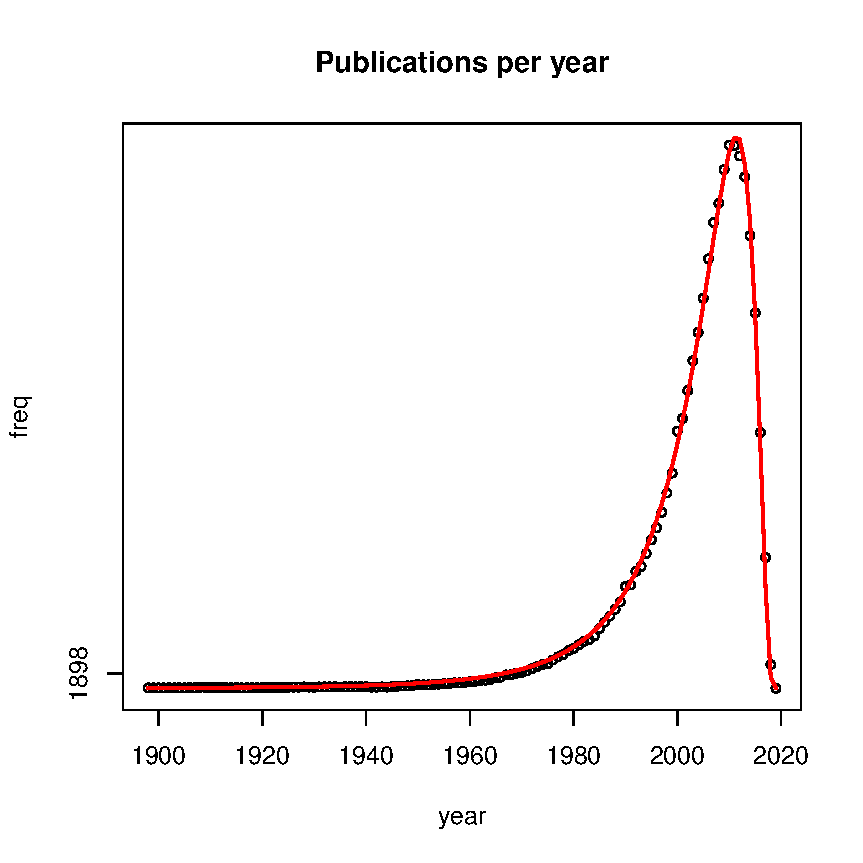
\includegraphics[width=95mm]{pubYear.pdf}}
\caption{Citation network: Distribution of works by years}\label{yeard}
\end{figure}

Figure~\ref{yeard}.  log normal distribution

\[ c\cdot \mbox{dlnorm}(2019-year,a,b) \]

$a = 2.543$,
$b = 0.7206$,
$c = 1.278 10^6$

\begin{figure}
%\includegraphics[width=43mm,viewport=100 40 405 550,clip=]{island2.pdf}
\centerline{
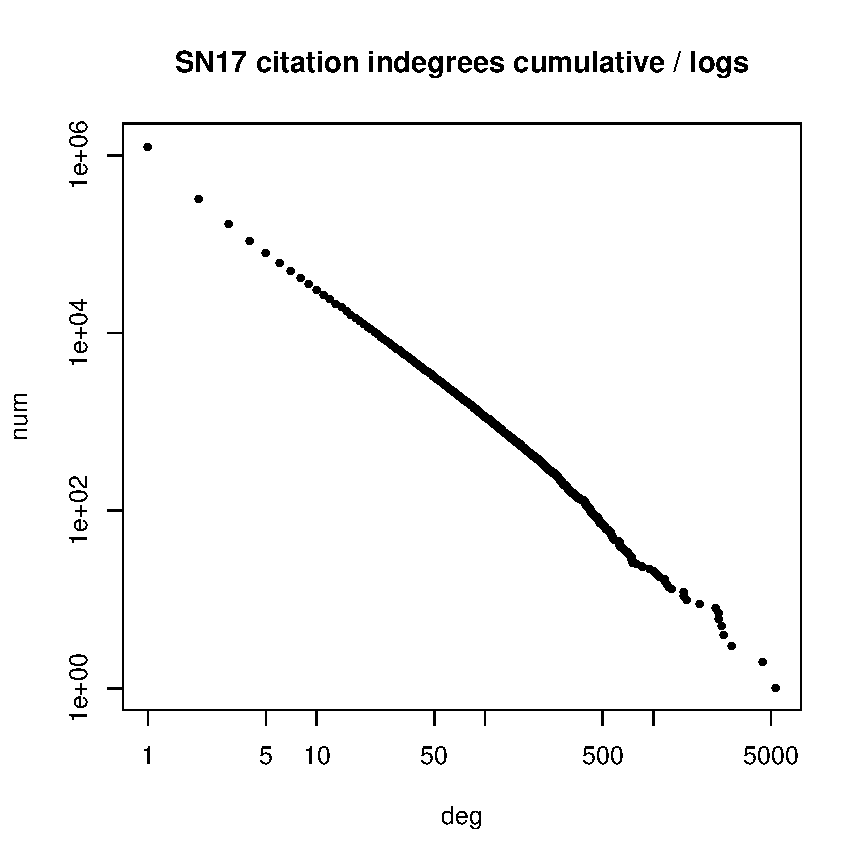
\includegraphics[width=0.45\textwidth]{CiteIndegCum.pdf} \qquad
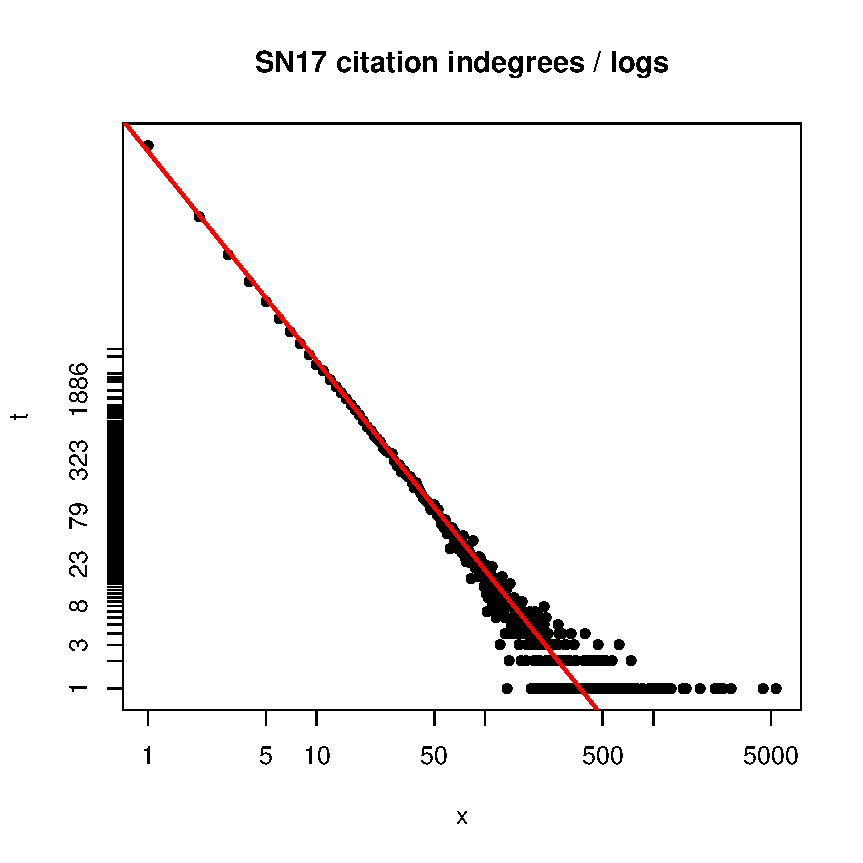
\includegraphics[width=0.45\textwidth]{CiteIndegplfit.pdf} }
\caption{Citation network: Indegree distribution}\label{cindeg}
\end{figure}

Figure~\ref{cindeg}.
The indegree distribution in citation network follows the \keyw{power law} $f = c \cdot n^{-\alpha}$.

Fitted $\alpha = 2.3007$, $c=749338$.


\begin{table}
\caption{Citation net:\label{mostcited} The most cited works - indegree}\medskip

\renewcommand{\arraystretch}{0.9}
%\small
\begin{tabular}{r|r|l||r|r|l}
i	& freq	& id	                                           & i	& freq & id \\ \hline
1& 	5348& 	WASSERMA\_S(1994):& 	31& 	734& 	NEWMAN\_M(2001)98:404	\\
2& 	4471& 	GRANOVET\_M(1973)78:1360& 	32& 	719& 	NEWMAN\_M(2010):	\\
3& 	2906& 	WATTS\_D(1998)393:440& 	33& 	701& 	PORTES\_A(1998)24:1	\\
4& 	2614& 	BARABASI\_A(1999)286:509& 	34& 	687& 	BLEI\_D(2003)3:993	\\
5& 	2561& 	FREEMAN\_L(1979)1:215& 	35& 	670& 	BURT\_R(2004)110:349	\\
6& 	2447& 	BOYD\_D(2007)13:210& 	36& 	654& 	HANSEN\_M(1999)44:82	\\
7& 	2429& 	MCPHERSO\_M(2001)27:415& 	37& 	639& 	PALLA\_G(2005)435:814	\\
8& 	2330& 	BURT\_R(1992):& 	38& 	634& 	CLAUSET\_A(2004)70:066111	\\
9& 	1886& 	COLEMAN\_J(1988)94:95& 	39& 	629& 	BONACICH\_P(1987)92:1170	\\
10& 	1572& 	NEWMAN\_M(2003)45:167& 	40& 	628& 	ERDOS\_P(1959)6:290	\\
11& 	1520& 	GIRVAN\_M(2002)99:7821& 	41& 	628& 	UZZI\_B(1997)42:35	\\
12& 	1510& 	PUTNAM\_R(2000):& 	42& 	628& 	ROGERS\_E(2003):	\\
13& 	1285& 	ALBERT\_R(2002)74:47& 	43& 	613& 	PUTNAM\_R(1993):	\\
14& 	1240& 	GRANOVET\_M(1985)91:481& 	44& 	593& 	BERKMAN\_L(1979)109:186	\\
15& 	1192& 	SCOTT\_J(2000):& 	45& 	583& 	ZACHARY\_W(1977)33:452	\\
16& 	1171& 	EVERETT\_M(2002):& 	46& 	572& 	BORGATTI\_S(2009)323:892	\\
17& 	1166& 	NEWMAN\_M(2004)69:026113& 	47& 	569& 	NEWMAN\_M(2001)64:025102	\\
18& 	1093& 	COLEMAN\_J(1990):& 	48& 	565& 	BURT\_R(2005):	\\
19& 	1058& 	STEINFIE\_C(2007)12:1143& 	49& 	561& 	ADLER\_P(2002)27:17	\\
20& 	1034& 	FORTUNAT\_S(2010)486:75& 	50& 	559& 	CHRISTAK\_N(2008)358:2249	\\
21& 	999& 	BORGATTI\_S(2002):& 	51& 	555& 	ROGERS\_E(1995):	\\
22& 	945& 	CHRISTAK\_N(2007)357:370& 	52& 	554& 	MILGRAM\_S(1967)1:61	\\
23& 	867& 	FREEMAN\_L(1977)40:35& 	53& 	553& 	BARON\_R(1986)51:1173	\\
24& 	854& 	HANNEMAN\_R(2005):& 	54& 	550& 	GRANOVET\_M(1978)83:1420	\\
25& 	800& 	LIN\_N(2001):& 	55& 	539& 	FISCHER\_C(1982):	\\
26& 	757& 	KAPLAN\_A(2010)53:59& 	56& 	537& 	BRIN\_S(1998)30:107	\\
27& 	756& 	BLONDEL\_V(2008):P10008& 	57& 	524& 	MARSDEN\_P(1990)16:435	\\
28& 	742& 	NAHAPIET\_J(1998)23:242& 	58& 	523& 	KEMP\_D(2003):137	\\
29& 	740& 	FORNELL\_C(1981)18:39& 	59& 	523& 	KLEINBER\_J(1999)46:604	\\
30& 	740& 	NEWMAN\_M(2006)103:8577& 	60& 	517& 	BOCCALET\_S(2006)424:175	\\ \hline
\end{tabular}
\end{table}

Table~\ref{mostcited}.

\begin{table}
\caption{Citation net: \label{maxciting} The most citing work -- outdegree}
\renewcommand{\arraystretch}{0.82}
\small
\begin{tabular}{r|r|l||r|r|l}
i&	freq& 	id&	i&	freq&	id	\\ \hline 
1& 	1572& 	CHAPMAN\_C(2016):1&	11& 	731& 	TSATSOU\_P(2014):1\\
2& 	1406& 	HRUSCHKA\_D(2010)5:1&	12& 	654& 	GOODALE\_E(2017):IX\\
3& 	1293& 	COWARD\_F(2015):1&	13& 	649& 	PEPPER\_G(2017)40:S0140525X1700190X\\
4& 	1254& 	FITZGERA\_P(2008):1&	14& 	632& 	STROM\_R(2012):1\\
5& 	1207& 	DAVIES\_N(2015):V&	15& 	613& 	SCHACHNE\_G(2015)23:49\\
6& 	1055& 	MARSH\_C(2009):1&	16& 	597& 	COSTA\_L(2011)60:329\\
7& 	942& 	YUS\_F(2011)213:1&	17& 	593& 	BRANDES\_U(2005)3418:1\\
8& 	929& 	BOCCALET\_S(2006)424:175&	18& 	586& 	ROBERTS\_J(2014):1\\
9& 	799& 	REEVES\_M(2017):1&	19& 	557& 	GUNTER\_B(2016):1\\
10& 	768& 	GROSS\_J(2007):1&	20& 	547& 	CASTELLA\_C(2009)81:591\\ \hline 
\end{tabular}
\end{table}

Table~\ref{maxciting}.

%\footnotesize
\begin{itemize}
\item MUIJS, D., Reynolds, D.,  CHAPMAN, C. (2015). Educational effectiveness and improvement research and practice: The emergence of the discipline. In The Routledge International Handbook of Educational Effectiveness and Improvement (pp. 33-56). Routledge.
\item  Hruschka, D. J. (2010). Friendship: Development, ecology, and evolution of a relationship (Vol. 5). Univ of California Press.
\item Coward, F., Hosfield, R., Pope, M.,  Wenban-Smith, F. (Eds.). (2015). Settlement, society and cognition in human evolution. Cambridge University Press.
\item Fitzgerald, P.,  Lambkin, B. (2008). Migration in Irish history 1607-2007. Springer.
\item Davies, N.B. Animal Social Networks Foreword. In: Krause, J., James, R., Franks, D. W., Croft, D. P. (Eds.). (2015). Animal social networks. Oxford University Press, USA.
\item Marsh, C. J. (2009). Key concepts for understanding curriculum. Routledge.
\end{itemize}



\subsection{Authors}

\begin{table}
\caption{WA net: \label{numpap} Authors with the largest number of papers -- indegree}
\renewcommand{\arraystretch}{0.9}
\begin{center}
\begin{tabular}{l|l|l||l|l|l}
Rank& 	Value& 	Id& 	Rank& 	Value& 	Id\\  \hline   
1& 	1169& 	WANG\_Y& 	21& 	552& 	KIM\_H\\ 
2& 	883& 	ZHANG\_Y& 	22& 	550& 	CHEN\_J\\ 
3& 	868& 	CHEN\_Y& 	23& 	536& 	LIU\_X\\ 
4& 	847& 	LI\_Y& 	24& 	533& 	WANG\_L\\ 
5& 	838& 	WANG\_X& 	25& 	509& 	LI\_H\\ 
6& 	819& 	ZHANG\_J& 	26& 	490& 	KIM\_Y\\ 
7& 	788& 	WANG\_J& 	27& 	485& 	ZHANG\_Z\\ 
8& 	786& 	LIU\_Y& 	28& 	474& 	WANG\_Z\\ 
9& 	766& 	LEE\_J& 	29& 	471& 	WANG\_S\\ 
10& 	765& 	LEE\_S& 	30& 	471& 	CHEN\_X\\ 
11& 	749& 	LI\_J& 	31& 	471& 	\textbf{NEWMAN\_M}\\ 
12& 	708& 	LI\_X& 	32& 	462& 	CHEN\_L\\ 
13& 	696& 	CHEN\_C& 	33& 	461& 	ZHANG\_L\\ 
14& 	690& 	KIM\_J& 	34& 	450& 	YANG\_Y\\ 
15& 	620& 	WANG\_H& 	35& 	450& 	ZHANG\_H\\ 
16& 	611& 	ZHANG\_X& 	36& 	432& 	WU\_J\\ 
17& 	611& 	LIU\_J& 	37& 	431& 	LEE\_H\\ 
18& 	570& 	CHEN\_H& 	38& 	420& 	LI\_Z\\ 
19& 	557& 	KIM\_S& 	39& 	420& 	WANG\_W\\ 
20& 	554& 	WANG\_C& 	40& 	417& 	LI\_L\\ \hline  
\end{tabular}
\end{center}
\end{table}

Table~\ref{numpap}.

The large number of Chinese authors in the list is a \href{https://en.wikipedia.org/wiki/List_of_common_Chinese_surnames}{"three Zhang, four Li"} effect. It is out of our resources to drill into this. We can only make a warning.



\begin{table}
\caption{WA net: \label{numpapout} Number of authors in works -- outdegree}
\renewcommand{\arraystretch}{0.9}
\begin{center}
\begin{tabular}{l|l|l||l|l|l}
outdeg&  	Freq&  	Freq\% &  	outdeg&   Freq &	Freq\%\\ \hline   
1&  	1239496&  	95.5566&  	21&  	4&  	0.0003\\
2&  	18637&  	1.4368&  	22&  	3&  	0.0002\\
3&  	16661&  	1.2844&  	23&  	4&  	0.0003\\
4&  	10617&  	0.8185&  	24&  	2&  	0.0002\\
5&  	5759&  	0.4440&  	25&  	1&  	0.0001\\
6&  	2802&  	0.2160&  	26&  	2&  	0.0002\\
7&  	1322&  	0.1019&  	27&  	5&  	0.0004\\
8&  	686&  	0.0529&  	28&  	2&  	0.0002\\
9&  	384&  	0.0296&  	29&  	1&  	0.0001\\
10&  	247&  	0.0190&  	31&  	3&  	0.0002\\
11&  	155&  	0.0119&  	36&  	1&  	0.0001\\
12&  	90&  	0.0069&  	41&  	1&  	0.0001\\
13&  	70&  	0.0054&  	42&  	1&  	0.0001\\
14&  	54&  	0.0042&  	43&  	1&  	0.0001\\
15&  	32&  	0.0025&  	48&  	1&  	0.0001\\
16&  	12&  	0.0009&  	53&  	1&  	0.0001\\
17&  	14&  	0.0011&  	126&  	1&  	0.0001\\
18&  	9&  	0.0007&  	  & 	 & 	\\
19&  	6&  	0.0005&  	 &	 &	\\
20&  	2&  	0.0002&  	&	 &	\\ \hline
SUM &     &              &       &  1297133 & 100  \\ \hline   
\end{tabular}
\end{center}
\end{table}

Table~\ref{numpapout}.


Works with the largest number of authors:

\begin{center}
\renewcommand{\arraystretch}{0.9}
\begin{tabular}{l|l|l|l|}
     Rank    & Freq & Id \\ \hline
         1   & 126  & WANG\_M(2016)34:828 \\
         2    & 53   & VASHISHT\_R(2012)7:0039808 \\ 
         3      & 48  & SNIJDERS\_T(2007)170:322 \\ 
         4     & 43  & GUSTAVSS\_A(2011)21:718  \\ 
         5    & 42   & DOLL\_L(1992)29:1 \\ 
         6   &41 &  MAGLIANO\_L(2006)15:219 \\ \hline
\end{tabular}
\end{center}


WA net: Works with the largest number of authors -- outdegree.

Sharing and community curation of mass spectrometry data with Global Natural Products Social Molecular Networking / Nature Biotechnology volume 34, pages 828–837 (2016)


Mingxun Wang, Jeremy J Carver, Vanessa V Phelan, Laura M Sanchez, Neha Garg, Yao Peng, Don Duy Nguyen, Jeramie Watrous, Clifford A Kapono, Tal Luzzatto-Knaan, Carla Porto, Amina Bouslimani, Alexey V Melnik, Michael J Meehan, Wei-Ting Liu, Max Crüsemann, Paul D Boudreau, Eduardo Esquenazi, Mario Sandoval-Calderón, Roland D Kersten, Laura A Pace, Robert A Quinn, Katherine R Duncan, Cheng-Chih Hsu, Dimitrios J Floros, Ronnie G Gavilan, Karin Kleigrewe, Trent Northen, Rachel J Dutton, Delphine Parrot, Erin E Carlson, Bertrand Aigle, Charlotte F Michelsen, Lars Jelsbak, Christian Sohlenkamp, Pavel Pevzner, Anna Edlund, Jeffrey McLean, Jörn Piel, Brian T Murphy, Lena Gerwick, Chih-Chuang Liaw, Yu-Liang Yang, Hans-Ulrich Humpf, Maria Maansson, Robert A Keyzers, Amy C Sims, Andrew R Johnson, Ashley M Sidebottom, Brian E Sedio, Andreas Klitgaard, Charles B Larson, Cristopher A Boya P, Daniel Torres-Mendoza, David J Gonzalez, Denise B Silva, Lucas M Marques, Daniel P Demarque, Egle Pociute, Ellis C O'Neill, Enora Briand, Eric J N Helfrich, Eve A Granatosky, Evgenia Glukhov, Florian Ryffel, Hailey Houson, Hosein Mohimani, Jenan J Kharbush, Yi Zeng, Julia A Vorholt, Kenji L Kurita, Pep Charusanti, Kerry L McPhail, Kristian Fog Nielsen, Lisa Vuong, Maryam Elfeki, Matthew F Traxler, Niclas Engene, Nobuhiro Koyama, Oliver B Vining, Ralph Baric, Ricardo R Silva, Samantha J Mascuch, Sophie Tomasi, Stefan Jenkins, Venkat Macherla, Thomas Hoffman, Vinayak Agarwal, Philip G Williams, Jingqui Dai, Ram Neupane, Joshua Gurr, Andrés M C Rodríguez, Anne Lamsa, Chen Zhang, Kathleen Dorrestein, Brendan M Duggan, Jehad Almaliti, Pierre-Marie Allard, Prasad Phapale, Louis-Felix Nothias, Theodore Alexandrov, Marc Litaudon, Jean-Luc Wolfender, Jennifer E Kyle, Thomas O Metz, Tyler Peryea, Dac-Trung Nguyen, Danielle VanLeer, Paul Shinn, Ajit Jadhav, Rolf Müller, Katrina M Waters, Wenyuan Shi, Xueting Liu, Lixin Zhang, Rob Knight, Paul R Jensen, Bernhard Ø Palsson, Kit Pogliano, Roger G Linington, Marcelino Gutiérrez, Norberto P Lopes, William H Gerwick, Bradley S Moore, Pieter C Dorrestein, Nuno Bandeira.




\begin{table}
\caption{WJ net: The most used journals -- indegree}\label{jourind}\medskip

\renewcommand{\arraystretch}{0.9}
%\small
\begin{tabular}{r|r|l||r|r|l}
Rank&   	Value&   	Id&   	Rank&   	Value&   	Id \\ \hline
1&   	7080&   	LECT NOTES COMPUT SC&   	31&   	1258&   	AM J PSYCHIAT\\   
2&   	3859&   	SOC SCI MED&   	32&   	1221&   	J BUS RES\\   
3&   	3408&   	J PERS SOC PSYCHOL&   	33&   	1217&   	MANAGE SCI\\   
4&   	2719&   	COMPUT HUM BEHAV&   	34&   	1185&   	ACAD MANAGE REV\\   
5&   	2631&   	SCIENCE&   	35&   	1182&   	J CONSULT CLIN PSYCH\\   
6&   	2602&   	AM J PUBLIC HEALTH&   	36&   	1151&   	ORGAN SCI\\   
7&   	2599&   	P NATL ACAD SCI USA&   	37&   	1150&   	ADDICTION\\   
8&   	2208&   	NATURE&   	38&   	1143&   	STRATEGIC MANAGE J\\   
9&   	2058&   	AM SOCIOL REV&   	39&   	1087&   	J GERONTOL B-PSYCHOL\\   
10&   	1945&   	PHYSICA A&   	40&   	1075&   	PEDIATRICS\\   
11&   	1815&   	ANIM BEHAV&   	41&   	1055&   	AM J EPIDEMIOL\\   
12&   	1778&   	JAMA-J AM MED ASSOC&   	42&   	1050&   	COMPUT EDUC\\   
13&   	1763&   	LANCET&   	43&   	1022&   	DEV PSYCHOL\\   
14&   	1759&   	SCIENTOMETRICS&   	44&   	1022&   	PSYCHOL BULL\\   
15&   	1734&   	AM J SOCIOL&   	45&   	1007&   	J ADOLESCENT HEALTH\\   
16&   	1703&   	ACAD MANAGE J&   	46&   	997&   	J MARKETING\\   
17&   	1632&   	LECT NOTES ARTIF INT&   	47&   	996&   	ARCH GEN PSYCHIAT\\   
18&   	1573&   	J APPL PSYCHOL&   	48&   	994&   	AIDS BEHAV\\   
19&   	1551&   	SOC NETWORKS&   	49&   	972&   	PERS INDIV DIFFER\\   
20&   	1509&   	AM ECON REV&   	50&   	949&   	PERS SOC PSYCHOL B\\   
21&   	1433&   	J MARRIAGE FAM&   	51&   	947&   	J BUS ETHICS\\   
22&   	1400&   	BRIT MED J&   	52&   	939&   	J MARKETING RES\\   
23&   	1399&   	CHILD DEV&   	53&   	925&   	INFORM SCIENCES\\   
24&   	1373&   	EXPERT SYST APPL&   	54&   	916&   	HARVARD BUS REV\\   
25&   	1365&   	NEW ENGL J MED&   	55&   	915&   	IEEE T KNOWL DATA EN\\   
26&   	1363&   	COMMUN ACM&   	56&   	901&   	DRUG ALCOHOL DEPEN\\   
27&   	1355&   	RES POLICY&   	57&   	900&   	WORLD DEV\\   
28&   	1279&   	GERONTOLOGIST&   	58&   	899&   	AM J PREV MED\\   
29&   	1275&   	BRIT J PSYCHIAT&   	59&   	895&   	ADDICT BEHAV\\   
30&   	1271&   	SOC FORCES&   	60&   	893&   	J CONSUM RES\\  \hline
\end{tabular}

\end{table}

Table~\ref{jourind}

\begin{table}
\caption{WK net: The most used keywords -- indegree}\label{keyind}\medskip


\renewcommand{\arraystretch}{0.9}
%\small
\begin{center}
\begin{tabular}{r|r|l||r|r|l}
Rank&  	Value&  	Id&  	Rank&  	Value&  	Id\\ \hline
1&  	51333&  	social&  	31&  	3485&  	structure\\
2&  	46191&  	network&  	32&  	3479&  	life\\
3&  	11751&  	analysis&  	33&  	3444&  	risk\\
4&  	10219&  	model&  	34&  	3358&  	research\\
5&  	8104&  	community&  	35&  	3143&  	learn\\
6&  	8090&  	use&  	36&  	3116&  	influence\\
7&  	7596&  	base&  	37&  	3054&  	student\\
8&  	7439&  	information&  	38&  	3054&  	impact\\
9&  	7061&  	health&  	39&  	3049&  	perspective\\
10&  	7023&  	behavior&  	40&  	3042&  	complex\\
11&  	6745&  	online&  	41&  	3024&  	theory\\
12&  	6087&  	networking&  	42&  	2859&  	organization\\
13&  	5833&  	media&  	43&  	2828&  	relationship\\
14&  	5404&  	support&  	44&  	2802&  	algorithm\\
15&  	5101&  	communication&  	45&  	2776&  	education\\
16&  	5013&  	study&  	46&  	2714&  	group\\
17&  	4759&  	datum&  	47&  	2704&  	mobile\\
18&  	4376&  	management&  	48&  	2698&  	tie\\
19&  	4372&  	internet&  	49&  	2695&  	adult\\
20&  	4164&  	knowledge&  	50&  	2633&  	approach\\
21&  	4126&  	user&  	51&  	2608&  	care\\
22&  	4023&  	facebook&  	52&  	2551&  	adolescent\\
23&  	3984&  	technology&  	53&  	2479&  	role\\
24&  	3907&  	site&  	54&  	2472&  	state\\
25&  	3888&  	web&  	55&  	2467&  	innovation\\
26&  	3855&  	self&  	56&  	2434&  	pattern\\
27&  	3784&  	graph&  	57&  	2385&  	effect\\
28&  	3676&  	performance&  	58&  	2339&  	people\\
29&  	3534&  	service&  	59&  	2333&  	trust\\
30&  	3512&  	dynamics&  	60&  	2332&  	family\\ \hline
\end{tabular}
\end{center}

\end{table}

Table~\ref{keyind}



\section{Citation network}  

%******************************************************************************

\subsection{Cite net: Boundary problem}


The network Cite has 1297133  nodes and 2753767 arcs.

\begin{table}
\caption{Citation network:  Boundary problem}\label{citeb}\medskip

\begin{center}
\begin{tabular}{r|r|r|r|r|}
 indeg &       Freq &    Freq\%  &  CumFreq &  CumFreq\% \\ \hline
 0     & 41954   &  3.2344     & 41954   &  3.2344  \\ 
1   &  933315  &  71.9521   &  975269  & 75.1865  \\
2   &  154895   & 11.9413   & 1130164  &  87.1278 \\
3   &  58141    & 4.4823   & 1188305   & 91.6101  \\ 
4   &  29885   & 2.3039  & 1218190  & 93.9140 \\  
5   &  17651   & 1.3608   & 1235841  & 95.2748  \\ \hline
\end{tabular}
\end{center}
\end{table}


Most of nodes are terminal $(DCr=0)$ or nodes cited only once (indegree=1). We decided (boundary problem) to include in our networks nodes with $DCr > 0$ or $\indeg > 2$ (partition boundary). They determine a subnetwork CiteB with  222 086 nodes and 1 521 434 arcs.

Table~{citeb}

\subsection{Making citation network acyclic}

The citation network CiteB has 41 nontrivial strong components (see Figure~\ref{citecomp}).
 
To get an acyclic network we applied the \keyw{preprint transformation} to CiteB. The resulting network CiteT has 222 189 nodes and 1 521 658 arcs. 

We computed the SPC weights on network arcs, and determined 
\begin{itemize}
\item CPM path (Main path) = 59 nodes
\item Key-routes = 127 nodes  
\item SPC link islands [Line weights] of sizes [20, 200] = 5 islands of 138, 65, 13, 12, and 11 nodes  
\item SPC node islands [Vertex weights] of sizs  [20, 200] = 1 island of 200 nodes
\end{itemize}

%\medskip 

% We computed the Probabilistic flow on weighted network, and determined node islands [Vertex weights] of size  [10, 200] = 200 nodes.


\begin{figure}
\begin{center}
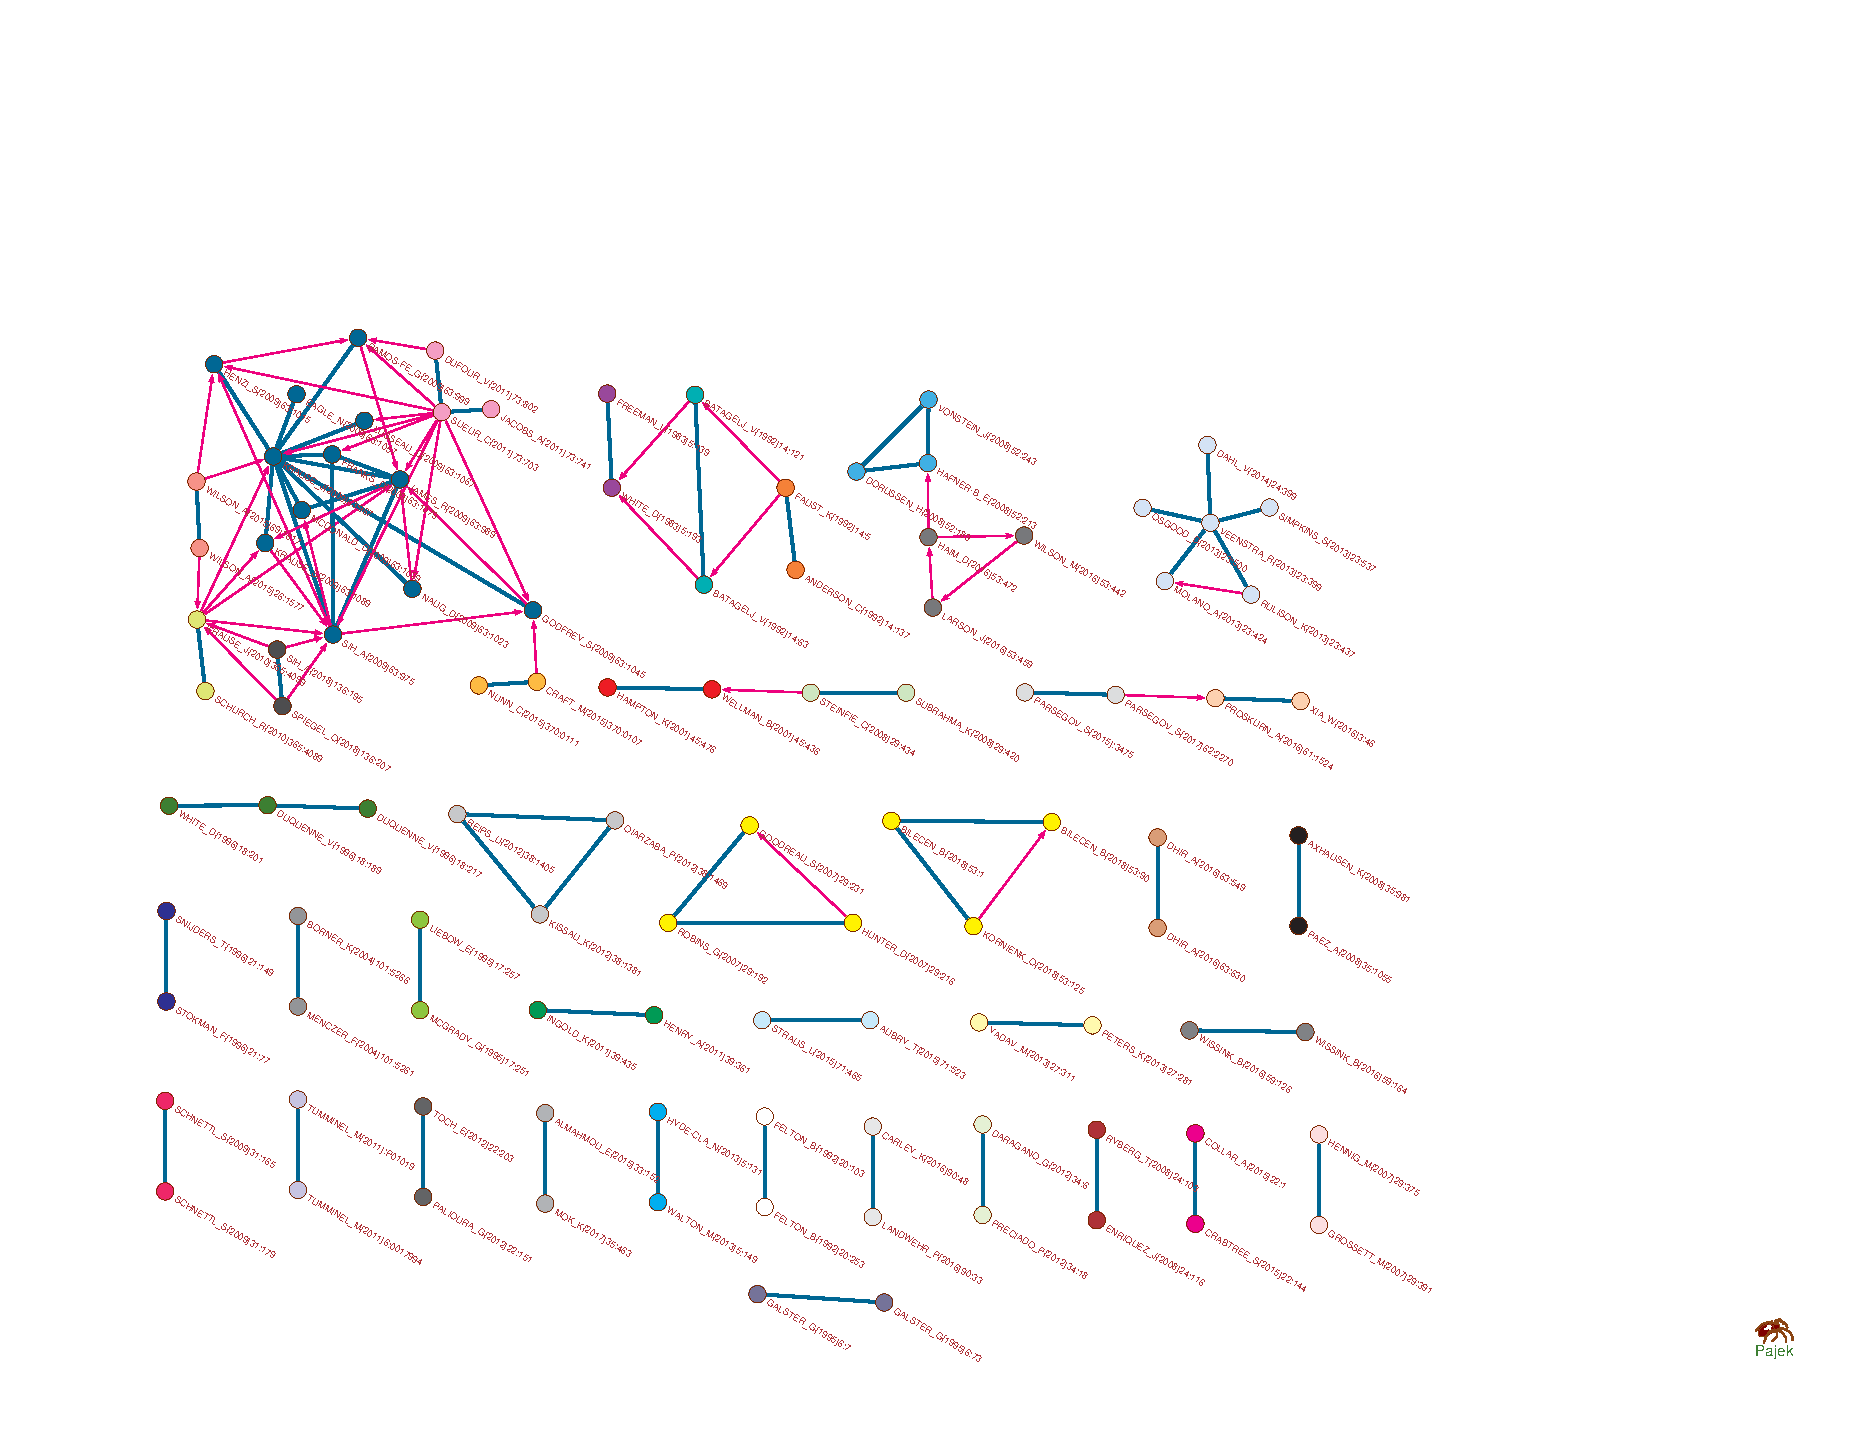
\includegraphics[width=\textwidth,viewport=75 34 690 535,clip=]{strong.pdf}
%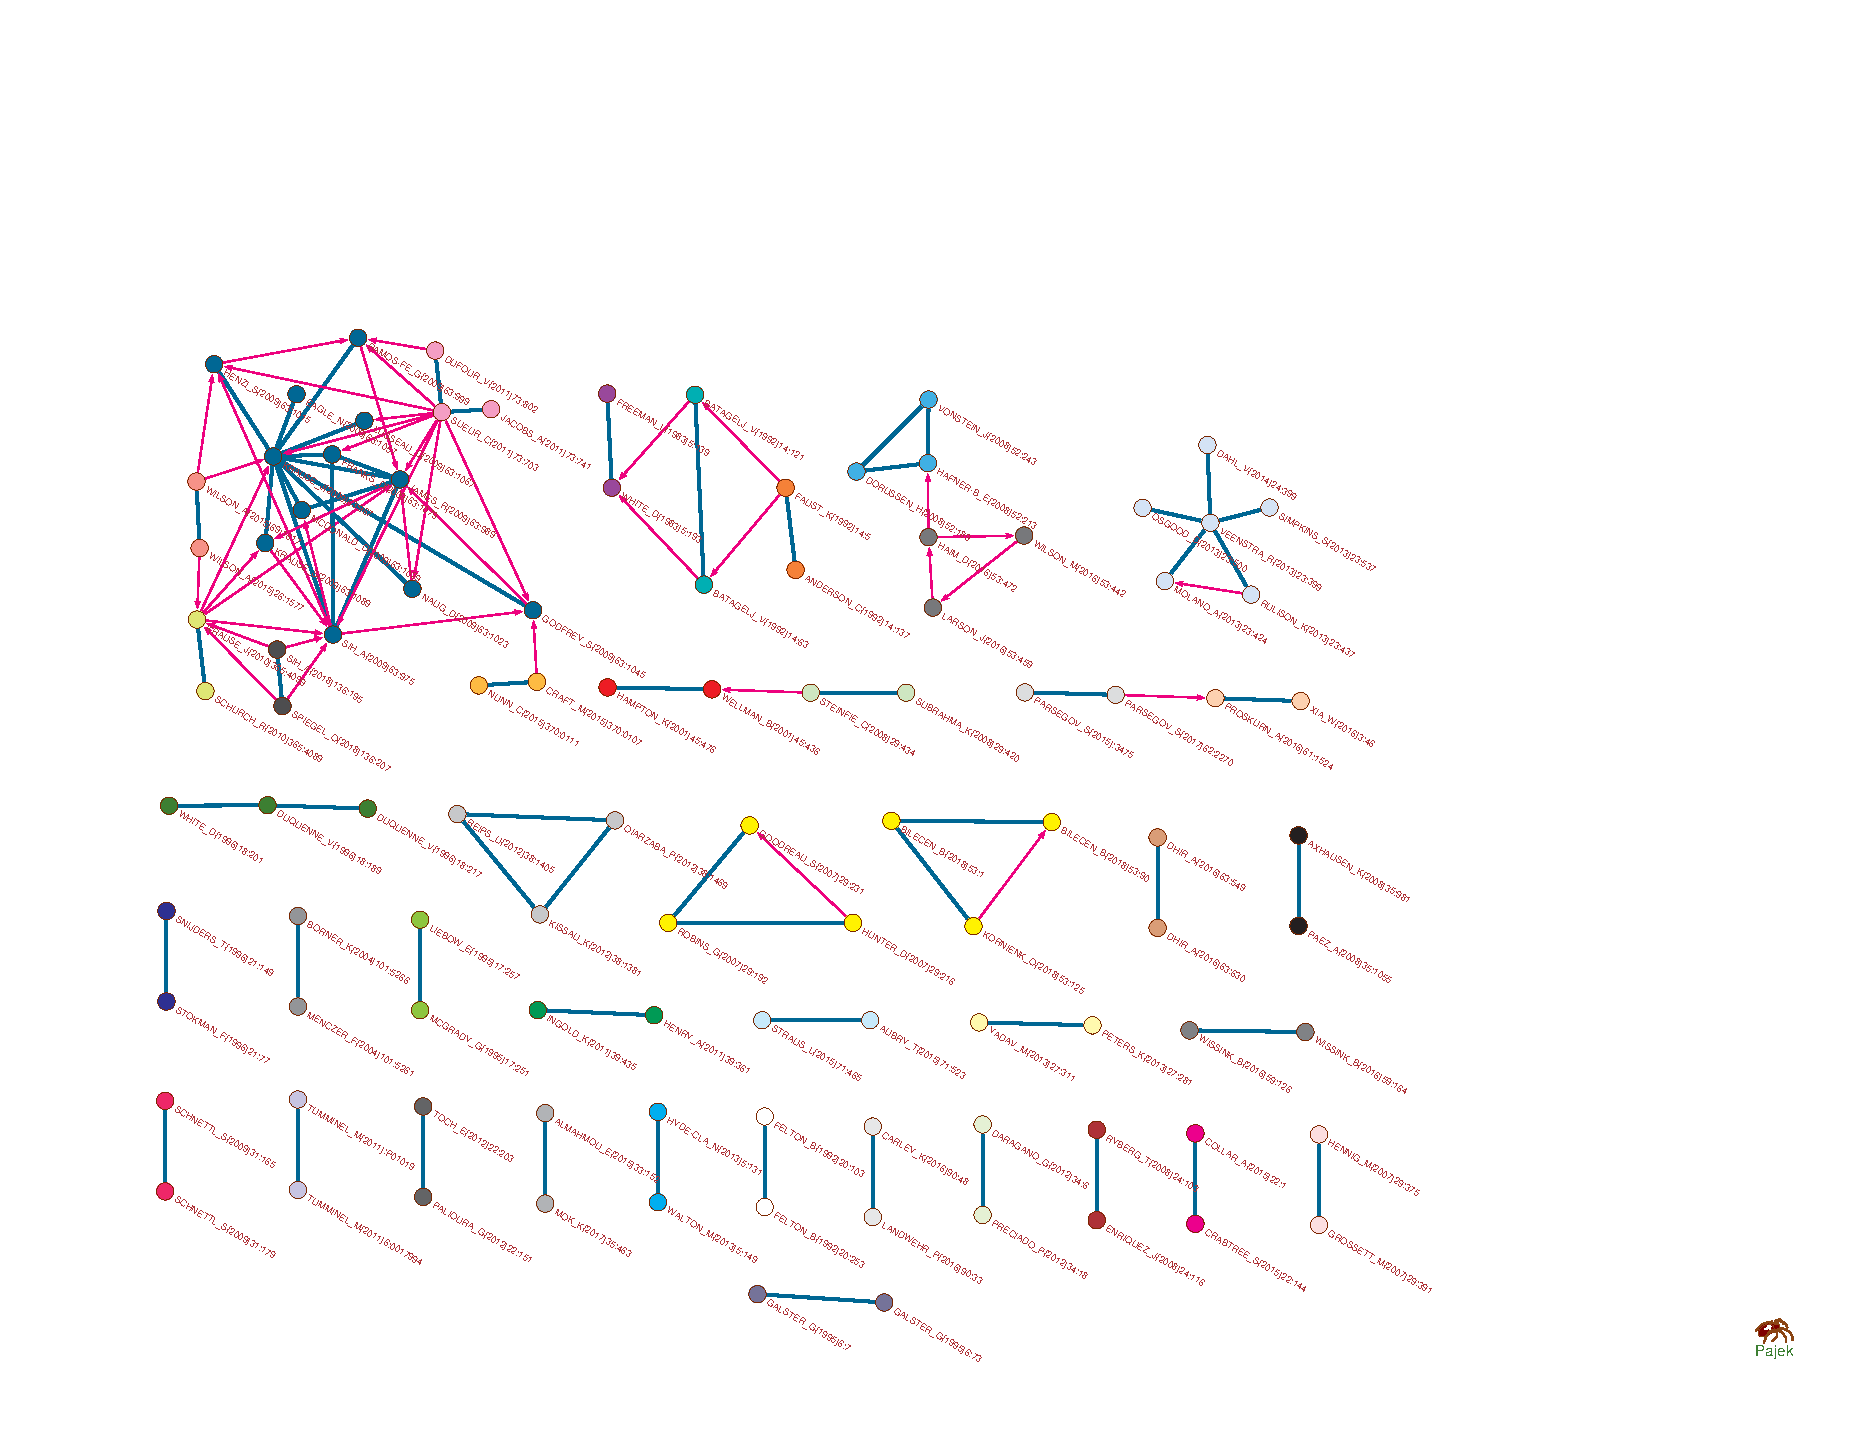
\includegraphics[width=100mm,viewport=90 320 670 535,clip=]{strong.pdf}
\end{center}
\caption{Strong components  \normalsize from SPC network} \label{citecomp}
\end{figure}

 Figure~\ref{citecomp}.

\subsection{Main Path, Key-Routes, Main Link Island}

\begin{figure}
\begin{center}

\includegraphics[width=11.7mm,viewport=120 27 235 682 ,clip=]{CPMpath.pdf}
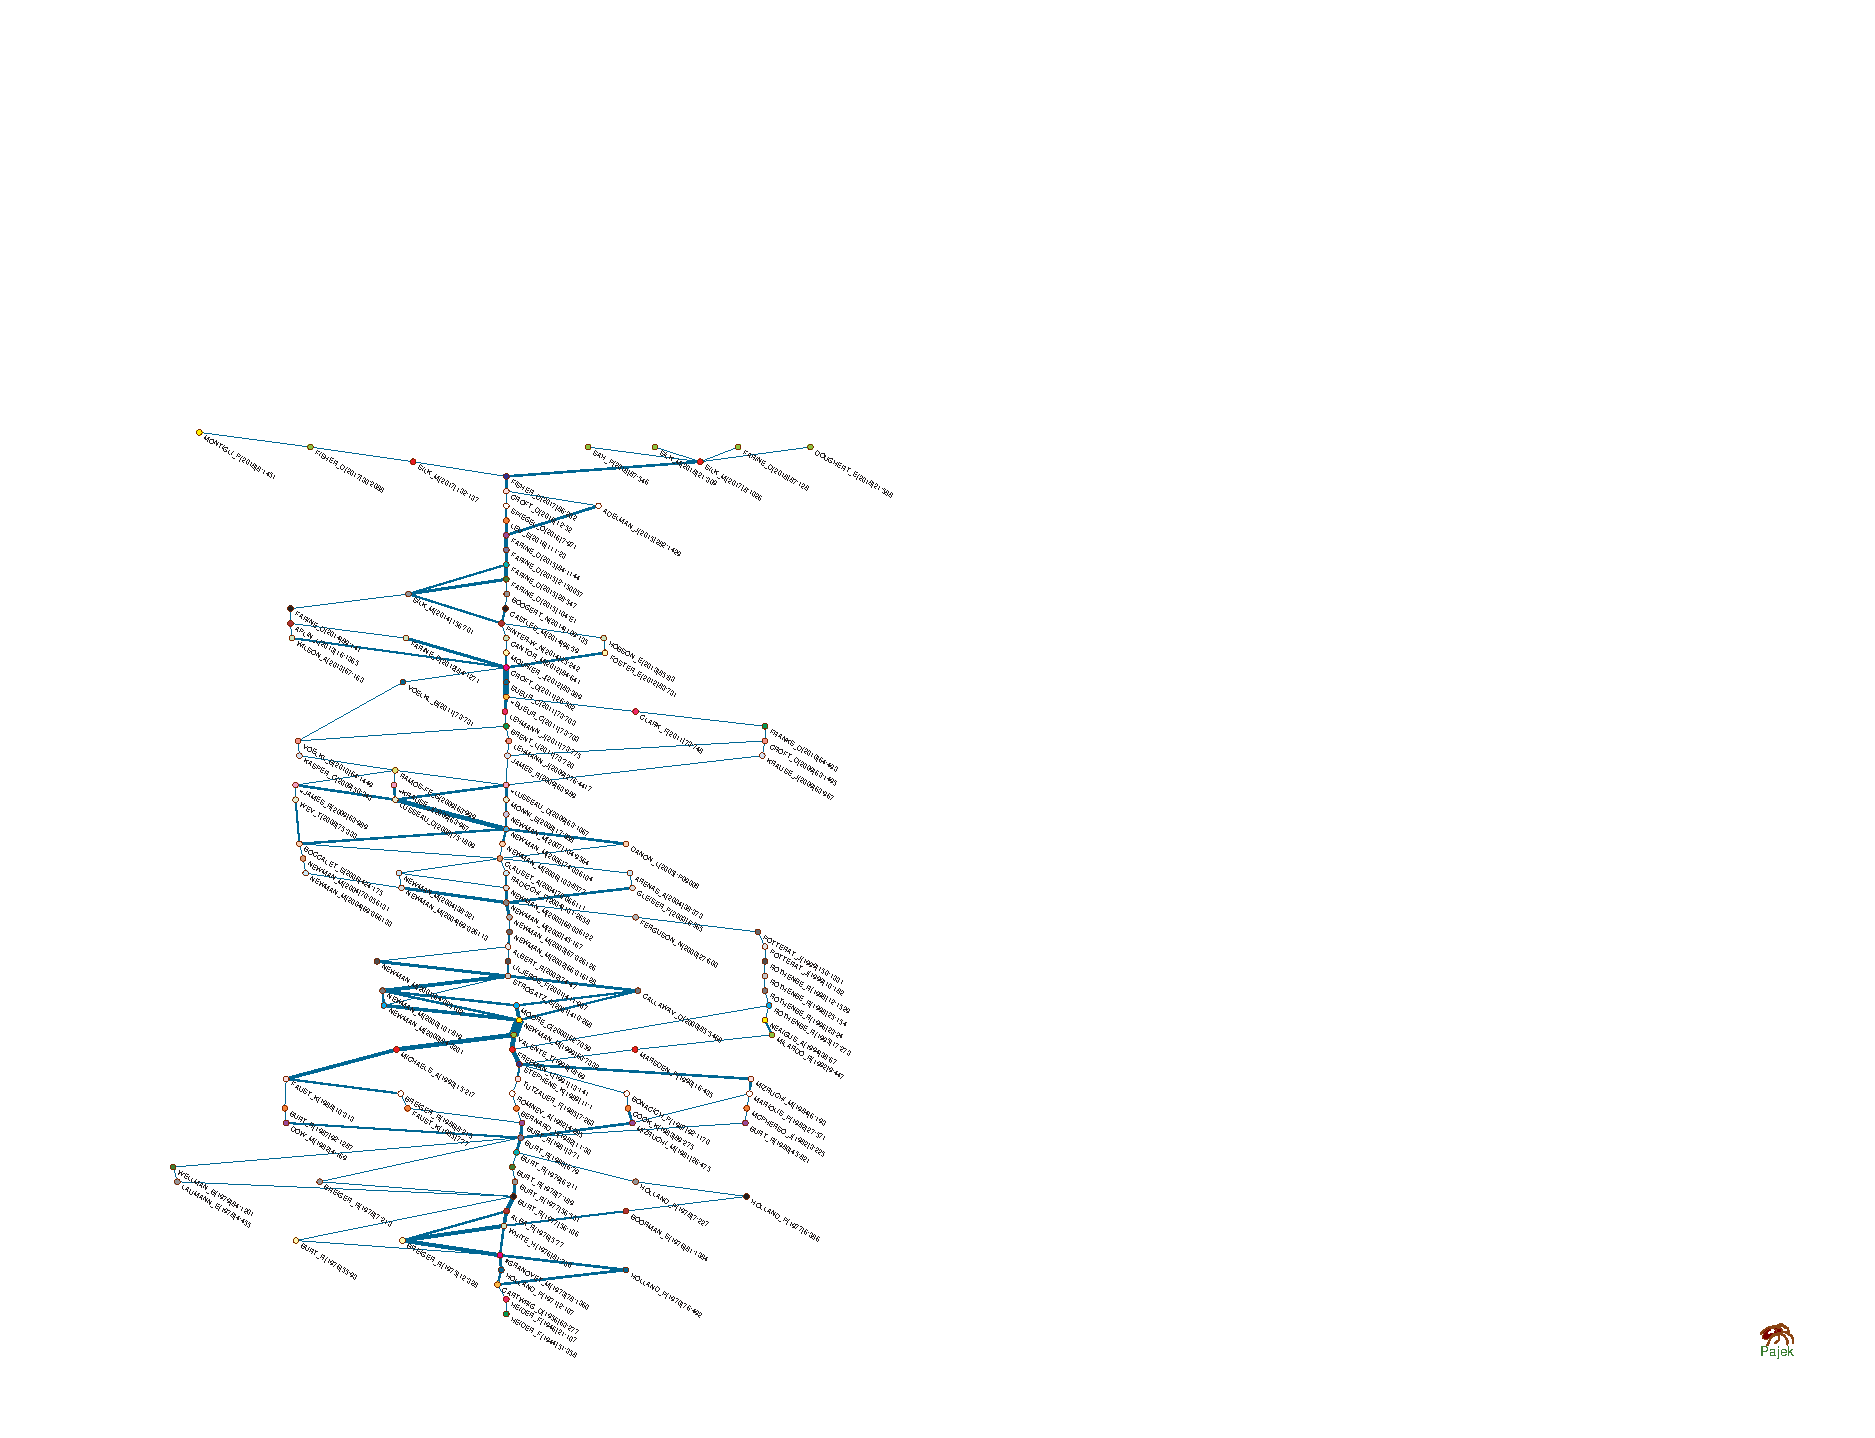
\includegraphics[width=53.3mm,viewport=75 37 440 590,clip=]{KeyRouteW.pdf}
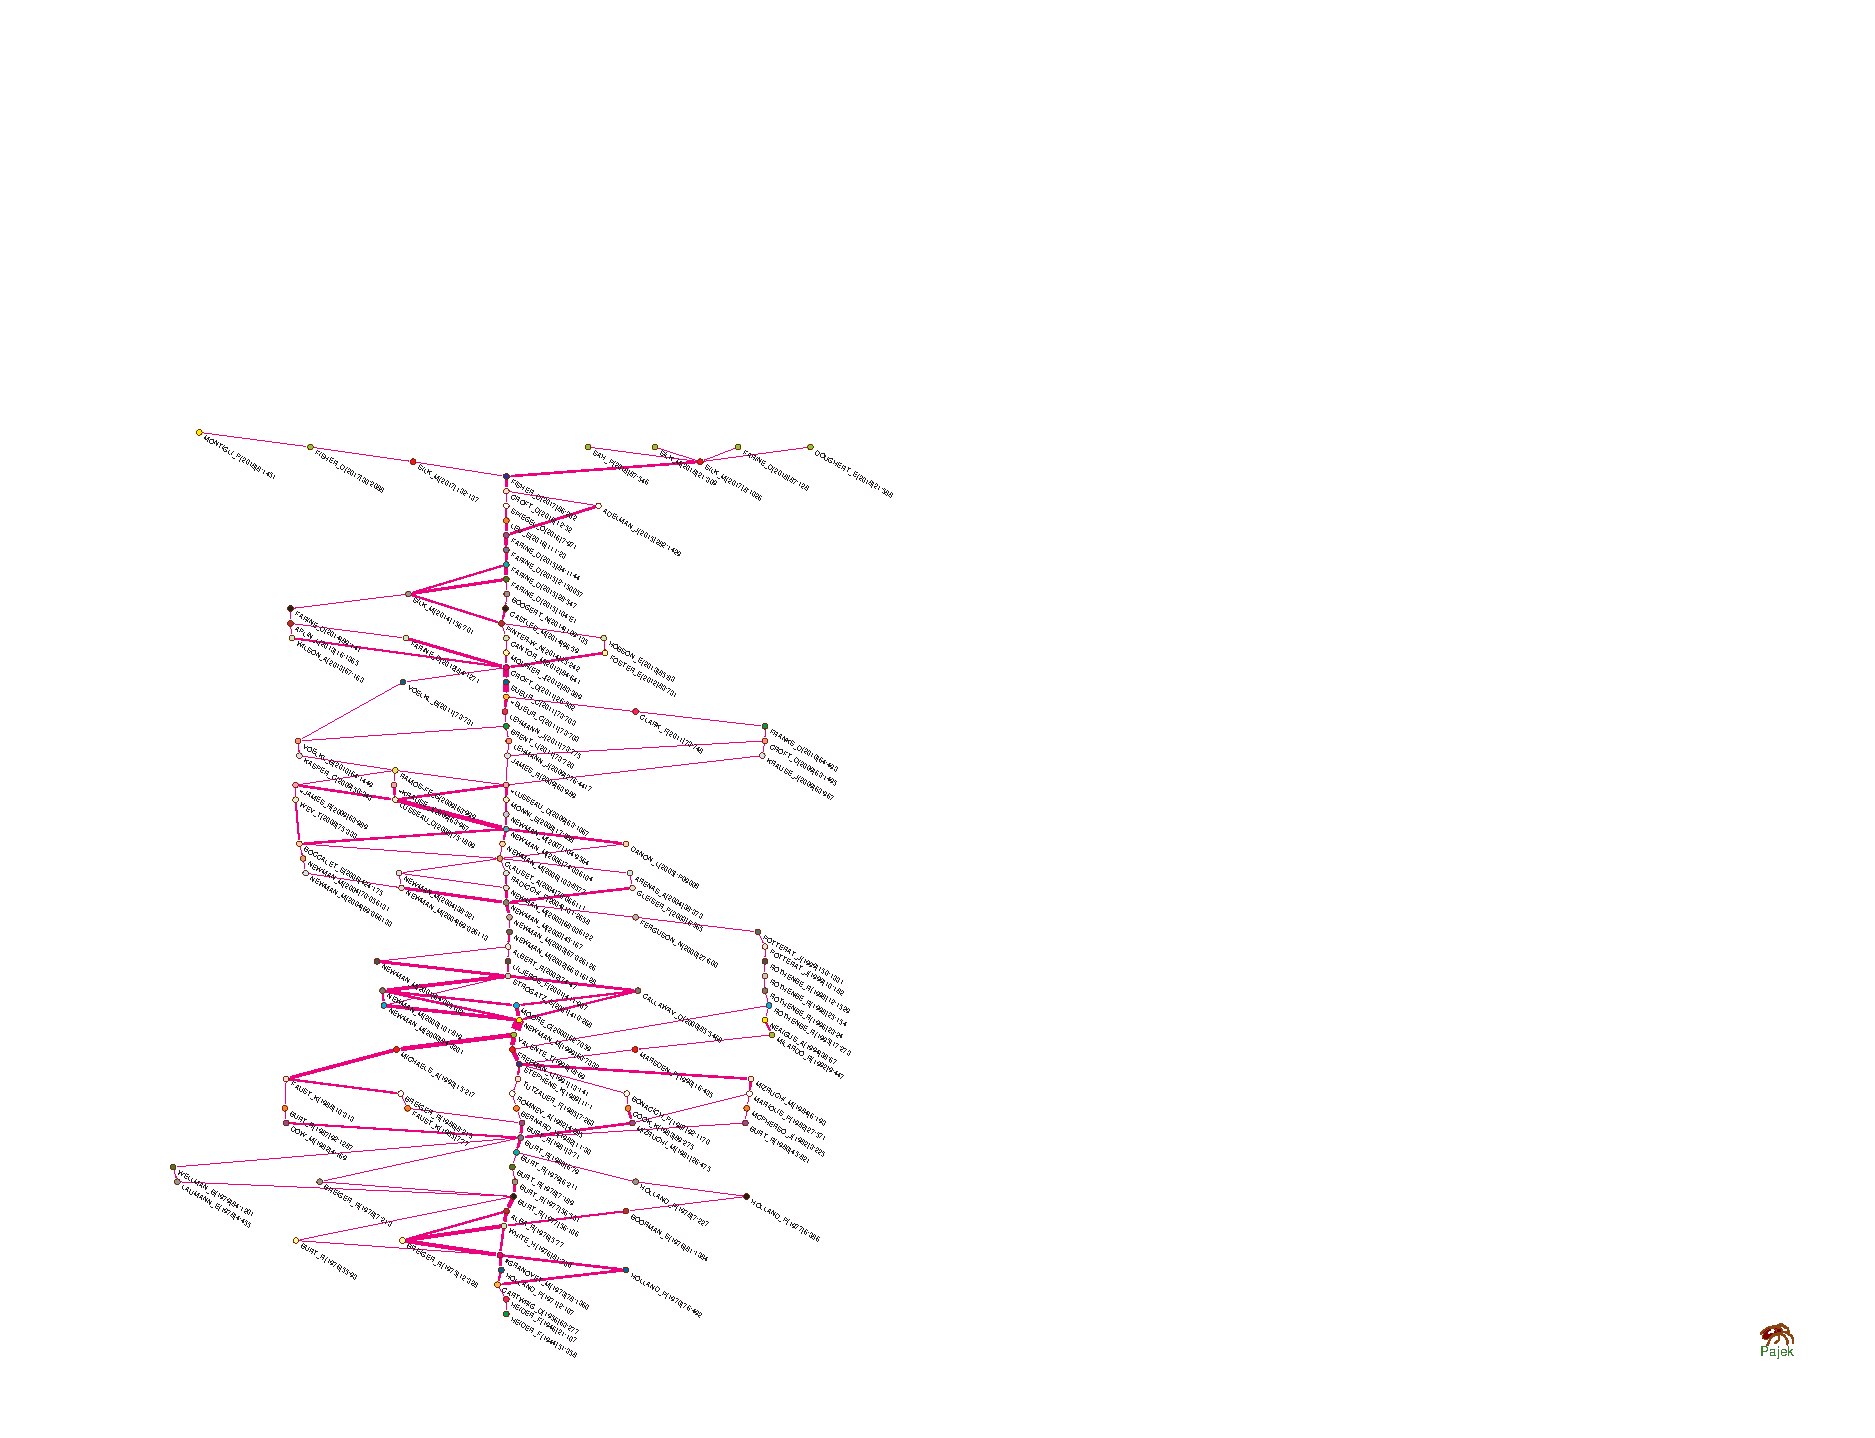
\includegraphics[width=65mm,viewport=182 34 633 490,clip=]{Island4w.pdf}
\end{center}
\caption{Main path, Key Routes, and Island 4 from SPC network} \label{citepaths}
\end{figure}

 Figure~\ref{citepaths}.
 
\begin{figure}
\begin{center}

\includegraphics[width=0.3\textwidth,viewport=118   28 235 262,clip=]{CPMpath.pdf}\qquad

\includegraphics[width=0.3\textwidth,viewport=118 239 235 416,clip=]{CPMpath.pdf}\qquad

\includegraphics[width=0.3\textwidth,viewport=118 394 235 681,clip=]{CPMpath.pdf}
\end{center}
\caption{Main path by fragments -- sociology, physics, biology}\label{mainFrag}
\end{figure}

 Figure~\ref{mainFrag}.
 
\begin{figure}
\begin{center}
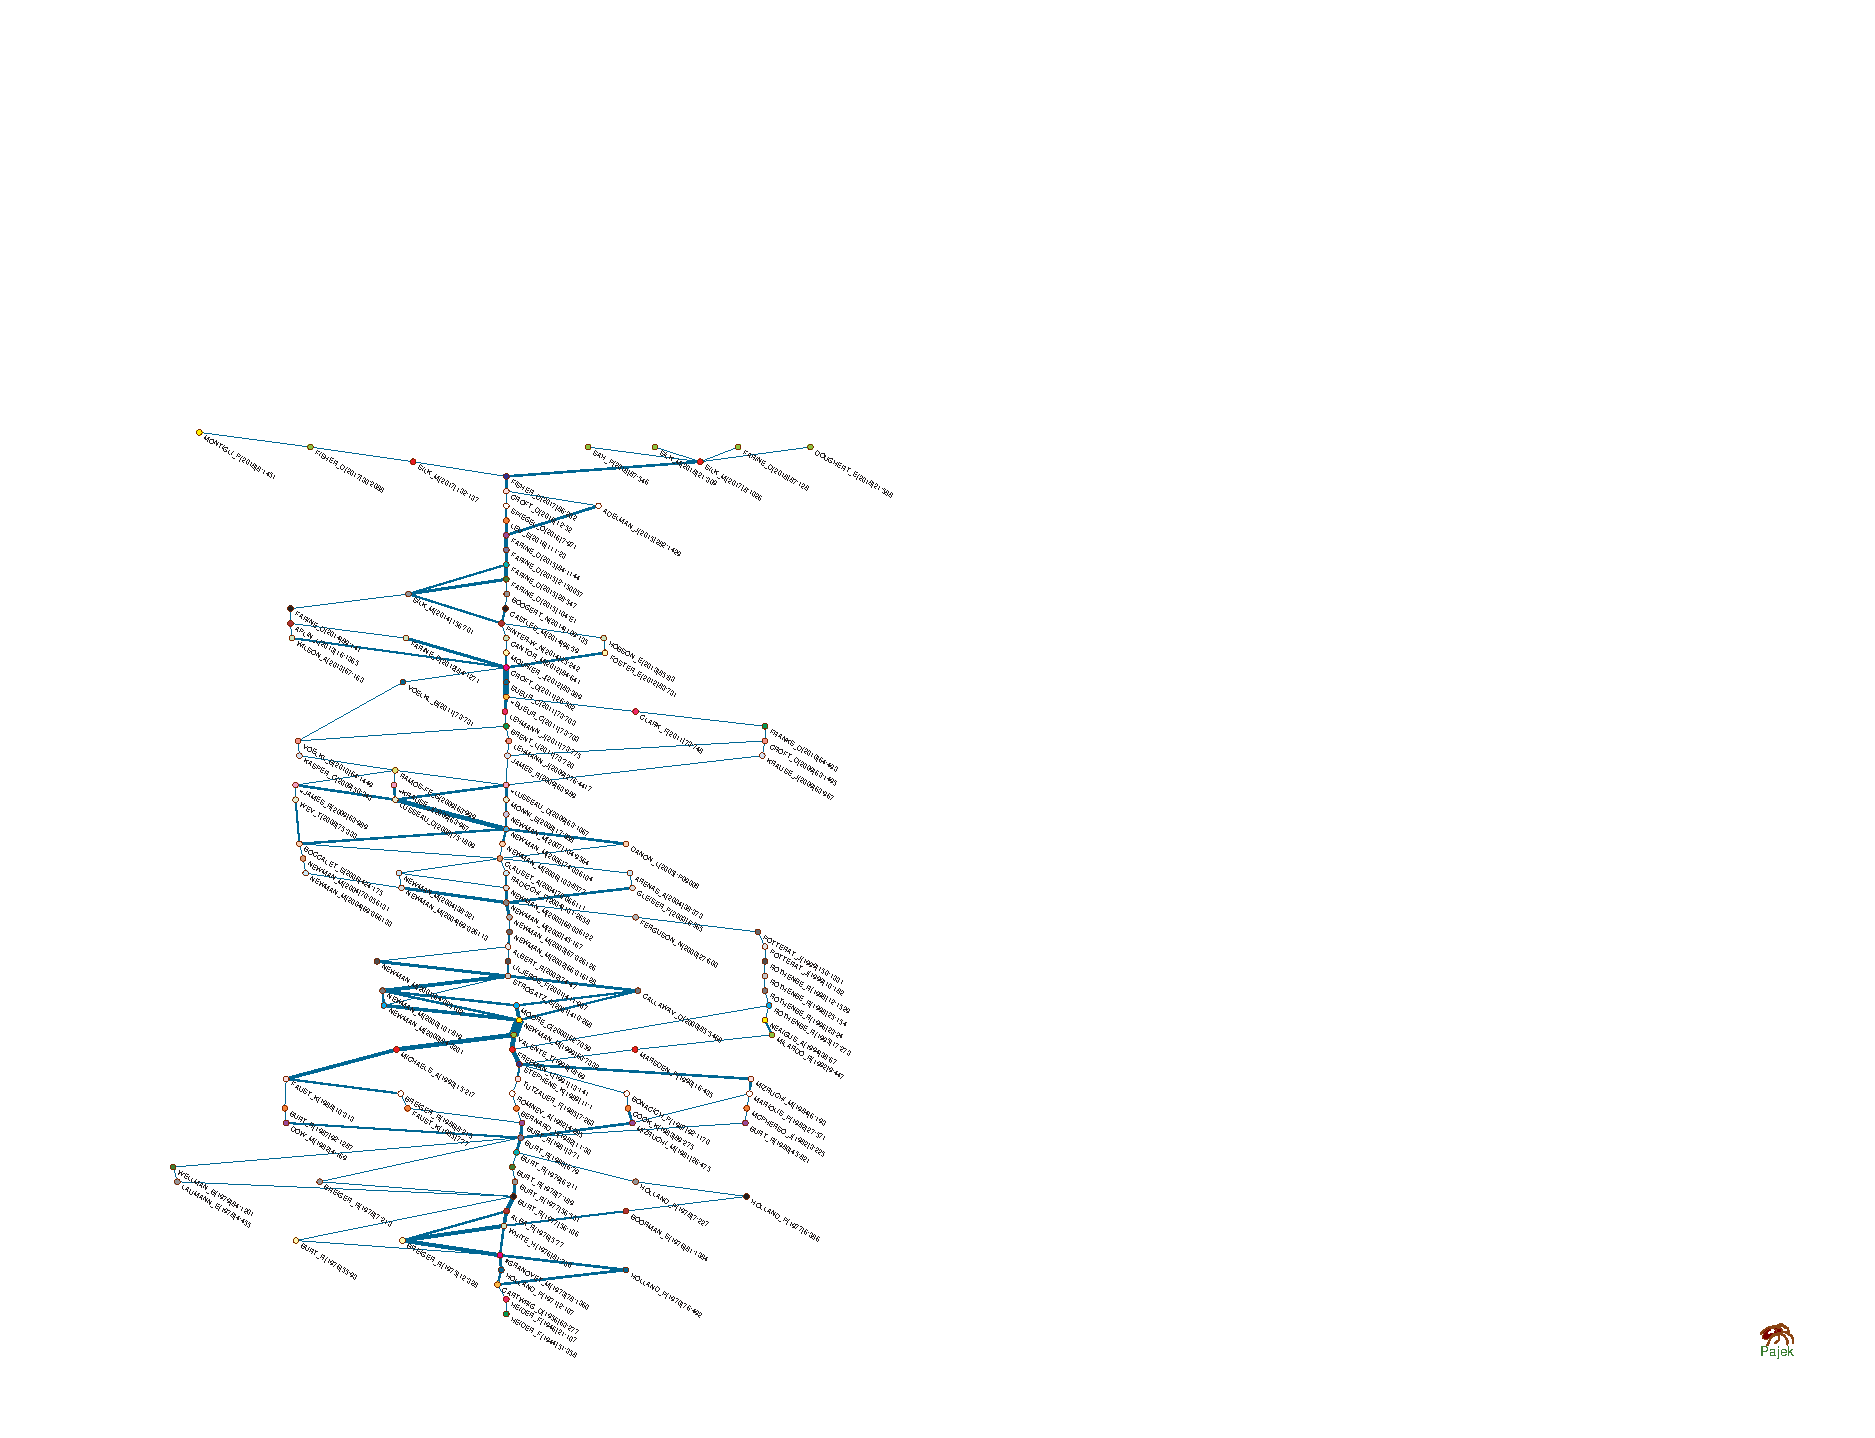
\includegraphics[width=\textwidth,viewport=75 37 440 540,clip=]{KeyRouteW.pdf}
\end{center}
\caption{ Key Routes} \label{keyRoute}
\end{figure}

 Figure~\ref{keyRoute}.
 

\begin{figure}
\begin{center}
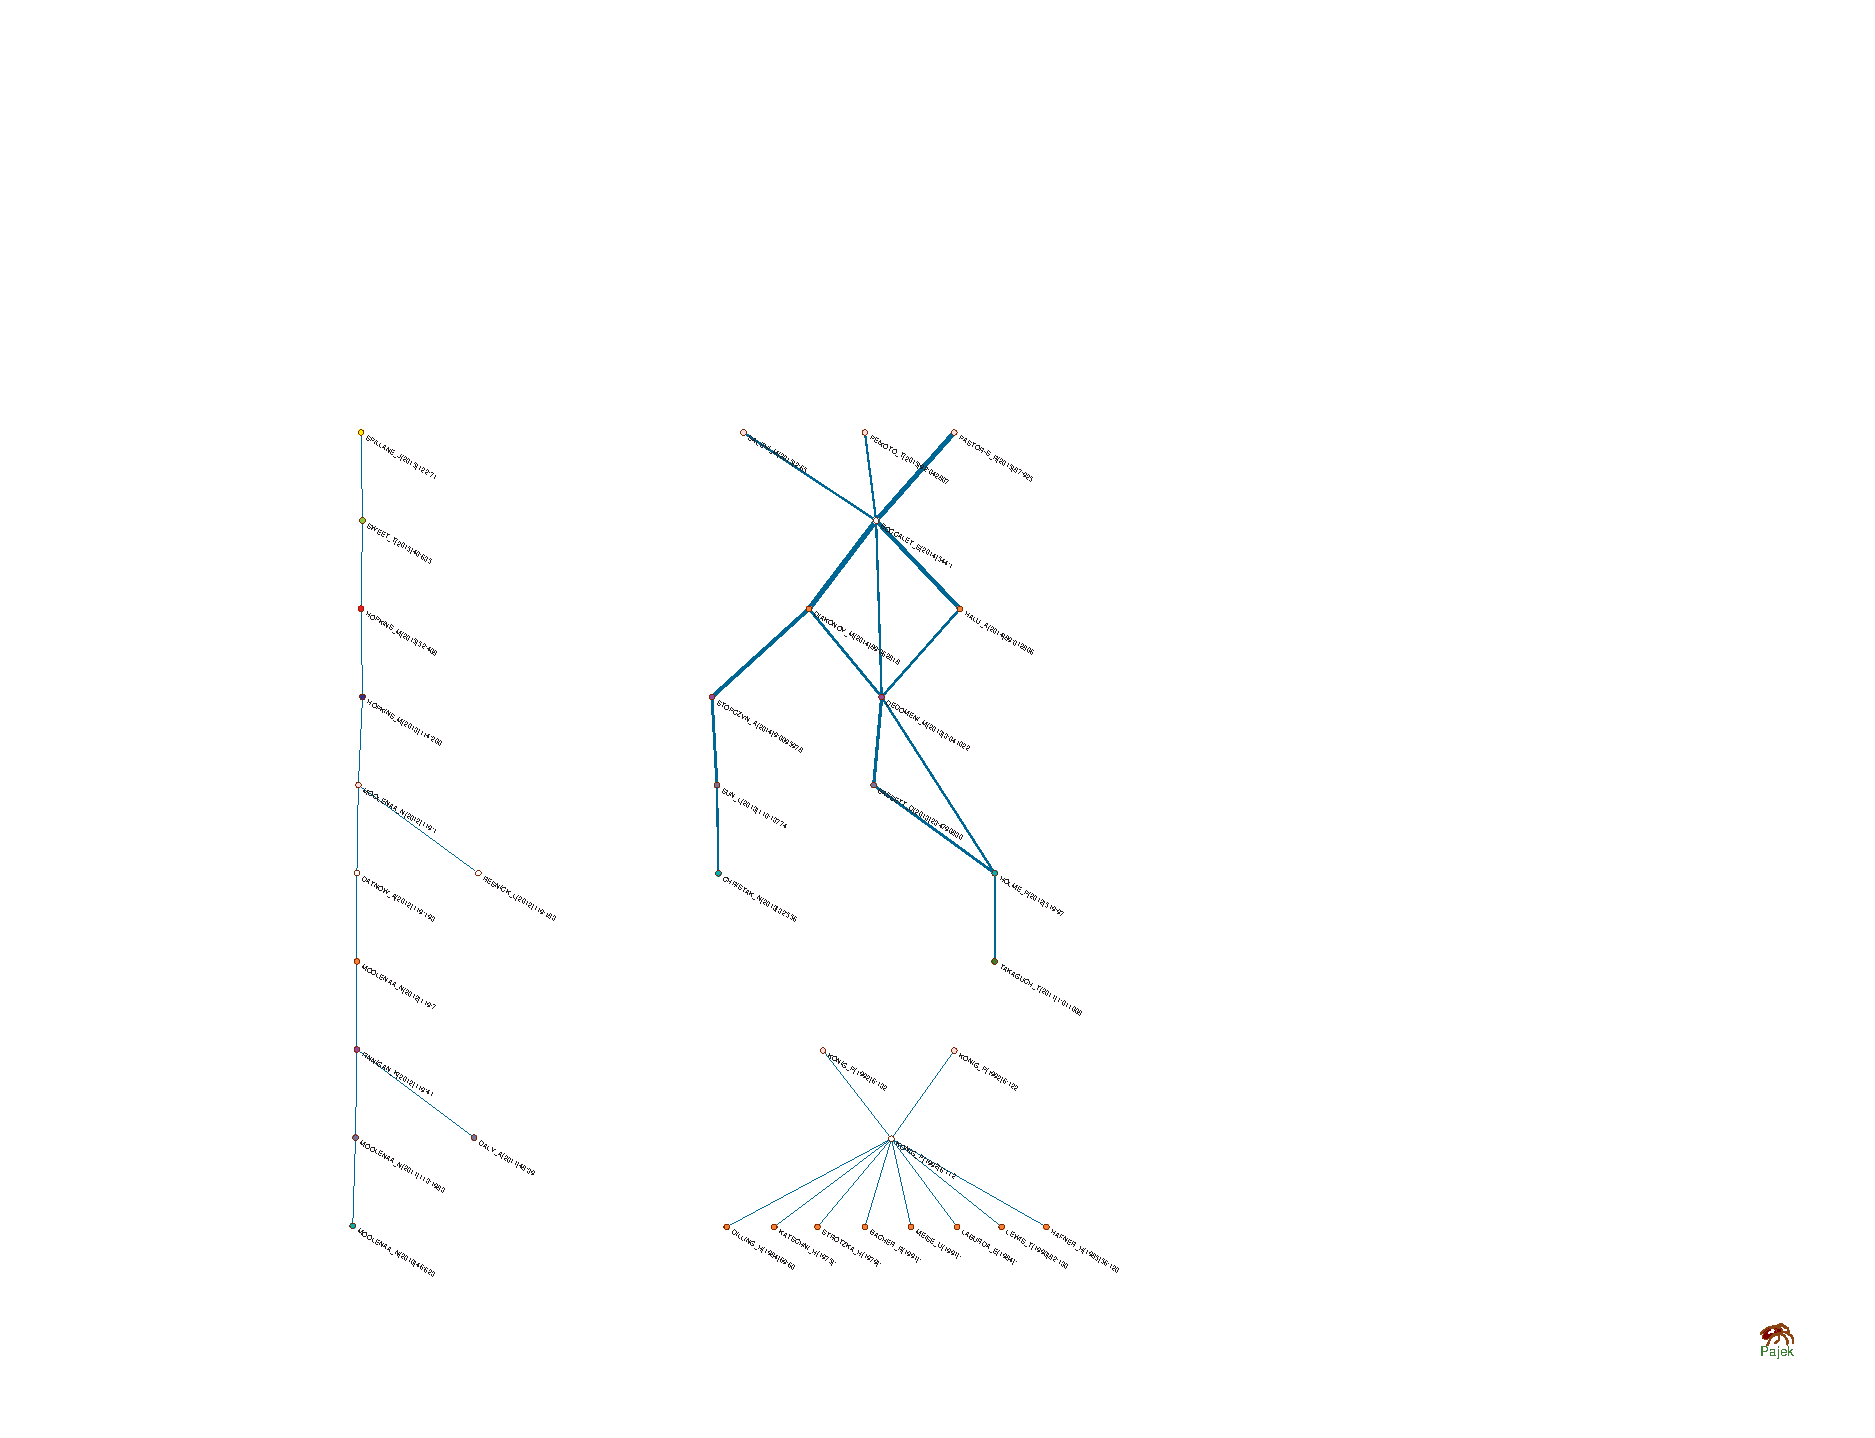
\includegraphics[width=78mm,viewport=160 75 540 488 ,clip=]{Island1-3w.pdf}
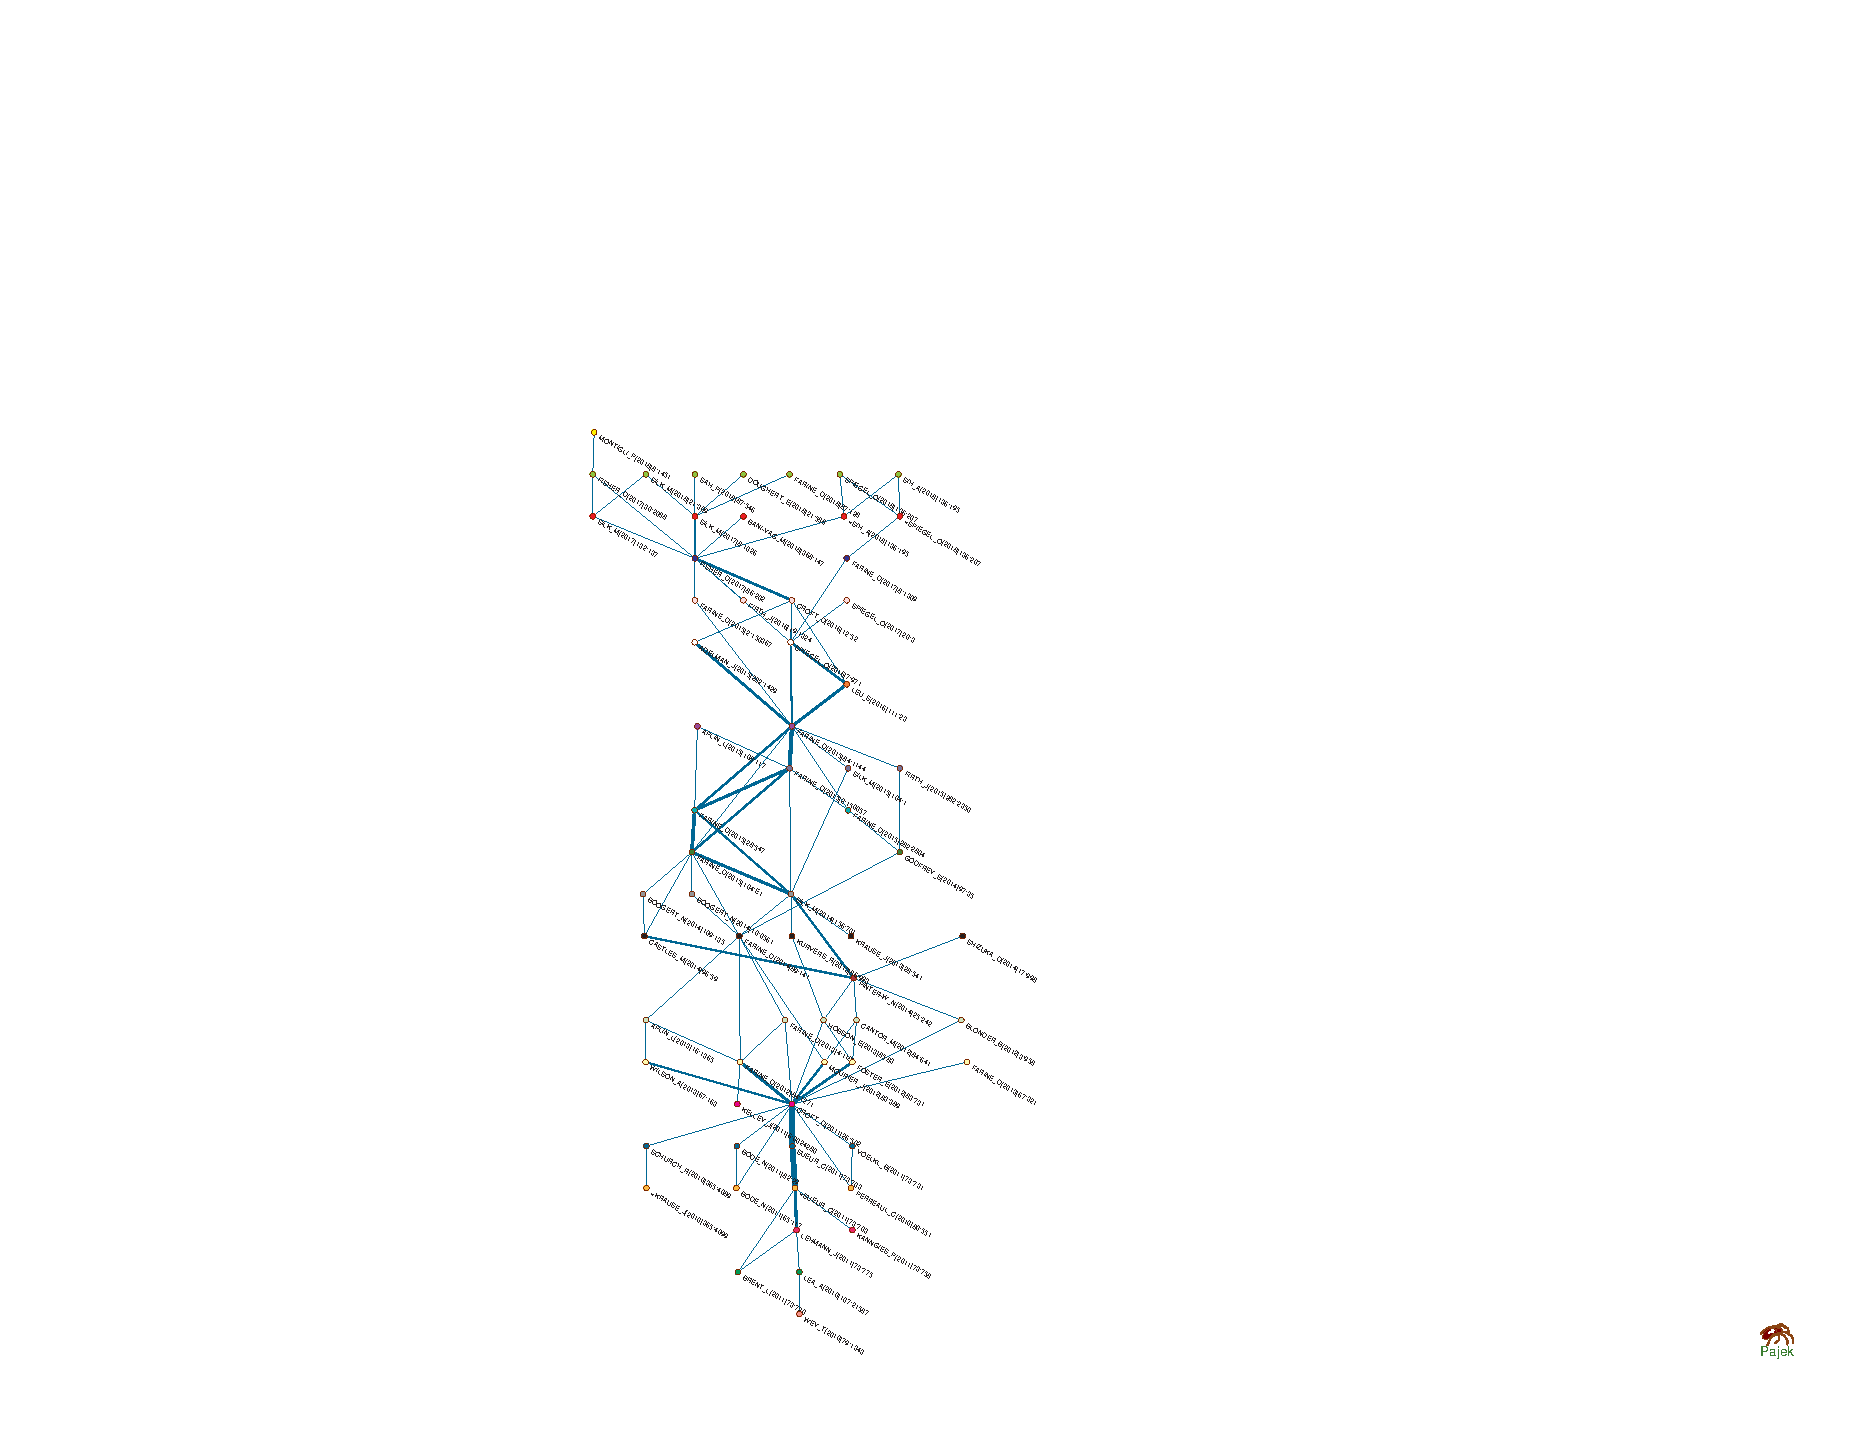
\includegraphics[width=42.9mm,viewport=280 37 500 488,clip=]{Island5w.pdf}
\end{center}
\caption{Islands 1-3, 5 e from SPC network} \label{citeislB}
\end{figure}

 Figure~\ref{citeislB}.

%******************************************************************************

\subsection{Probabilistic flow}


\begin{table}
\caption{Most important works  from Probabilistic  Flow network}\label{pFlow}\medskip

\small
\renewcommand{\arraystretch}{0.9}
\small
\begin{tabular}{c|c|l||c|c|l|l}
Rank&   	Value&   	Id&   	Rank&   	Value&   	Id\\ \hline
1&   	4691&   	WASSERMA\_S(1994):&   	31&   	545&   	BLONDEL\_V(2008):P10008\\
2&   	2941&   	WATTS\_D(1998)393:440&   	32&   	527&   	KATZ\_L(1953)18:39\\
3&   	2676&   	GRANOVET\_M(1973)78:1360&   	33&   	526&   	NEWMAN\_M(2010):\\
4&   	2445&   	BOYD\_D(2007)13:210&   	34&   	520&   	STROGATZ\_S(2001)410:268\\
5&   	2241&   	BARABASI\_A(1999)286:509&   	35&   	517&   	PALLA\_G(2005)435:814\\
6&   	1926&   	FREEMAN\_L(1979)1:215&   	36&   	499&   	CLAUSET\_A(2004)70:066111\\
7&   	1396&   	GIRVAN\_M(2002)99:7821&   	37&   	497&   	ERDOS\_P(1960)5:17\\
8&   	1299&   	NEWMAN\_M(2003)45:167&   	38&   	488&   	ROGERS\_E(2003):\\
9&   	1227&   	MCPHERSO\_M(2001)27:415&   	39&   	485&   	NEWMAN\_M(2006)103:8577\\
10&   	1158&   	ALBERT\_R(2002)74:47&   	40&   	481&   	COLEMAN\_J(1990):\\
11&   	1105&   	SCOTT\_J(2000):&   	41&   	478&   	BRIN\_S(1998)30:107\\
12&   	1098&   	BURT\_R(1992):&   	42&   	477&   	AMARAL\_L(2000)97:11149\\
13&   	1045&   	MILGRAM\_S(1967)1:61&   	43&   	475&   	ERDOS\_P(1959)6:290\\
14&   	1013&   	NEWMAN\_M(2004)69:026113&   	44&   	465&   	WATTS\_D(1999):\\
15&   	928&   	KAPLAN\_A(2010)53:59&   	45&   	462&   	LAVE\_J(1991):\\
16&   	878&   	FREEMAN\_L(1977)40:35&   	46&   	460&   	KLEINBER\_J(1999)46:604\\
17&   	852&   	PUTNAM\_R(2000):&   	47&   	449&   	SCOTT\_J(1991):\\
18&   	847&   	COLEMAN\_J(1988)94:95&   	48&   	446&   	BOLLOBAS\_B(1985):\\
19&   	835&   	BLEI\_D(2003)3:993&   	49&   	442&   	PAGE\_L(1999):\\
20&   	742&   	GRANOVET\_M(1985)91:481&   	50&   	440&   	NEWMAN\_M(2001)64:025102\\
21&   	731&   	CHRISTAK\_N(2007)357:370&   	51&   	436&   	NEWMAN\_M(2004)69:066133\\
22&   	727&   	EVERETT\_M(2002):&   	52&   	431&   	REDNER\_S(1998)4:131\\
23&   	726&   	NEWMAN\_M(2001)98:404&   	53&   	429&   	CHRISTAK\_N(2008)358:2249\\
24&   	719&   	ALBERT\_R(1999)401:130&   	54&   	424&   	ADOMAVIC\_G(2005)17:734\\
25&   	701&   	O'REILLY\_T(2005):&   	55&   	424&   	KEMP\_D(2003):137\\
26&   	669&   	BORGATTI\_S(2002):&   	56&   	423&   	DOMINGOS\_P(2001):57\\
27&   	667&   	FORTUNAT\_S(2010)486:75&   	57&   	423&   	MITCHELL\_J(1969):\\
28&   	633&   	HANNEMAN\_R(2005):&   	58&   	415&   	ALBERT\_R(2000)406:378\\
29&   	569&   	STEINFIE\_C(2007)12:1143&   	59&   	415&   	GLASER\_B(1967):\\
30&   	549&   	ZACHARY\_W(1977)33:452&   	60&   	410&   	ROGERS\_E(1995):\\ \hline
\end{tabular}

\end{table}

Table~\ref{pFlow}.

%******************************************************************************

\subsection{Comparisions}

\begin{table}
\caption{Cite net Overlapping of components} \label{compareA}\medskip
\small

\renewcommand{\arraystretch}{0.9}
\small
\begin{tabular}{c|l|l|l|l|}
i&   	name & title & journal & comp \\ \hline 
1&   	Granovet M &   	 Strength of weak ties&   	amer j sociol&   	1, 2, 4, 5, 6\\
2&   	Newman M&   	 The structure and function of complex networks&   	siam rev&   	1, 2, 4, 5, 6\\
3&   	Albert R&   	 Statistical mechanics of complex networks&   	rev mod phys&   	1, 2, 4, 5, 6\\
4&   	Boccaletti S&   	 Complex networks: structure and dynamics&   	phys rept&   	1, 2, 4, 5, 6\\
5&   	White H&   	 Soc. str. from mult. nets. Blockmodels &   	amer j sociol&   	1, 2, 4, 5, 6\\
6&   	Newman M&   	 Clustering and pref.l attach. in growing nets&   	phys rev e&   	1, 2, 4, 5, 6\\
7&   	Newman M&   	 Finding and evaluating comm. struct. in nets&   	phys rev e&   	1, 2, 4, 5, 6\\
8&   	Newman M&   	 Mixing patterns in networks&   	phys rev e&   	1, 2, 4, 5, 6\\
9&   	Strogatz S&   	 Exploring complex networks&   	nature&   	1, 2, 4, 5, 6\\
10&   	Newman M&   	 Detecting community structure in nets&   	eur phys j b&   	1, 2, 4, 5, 6\\
11&   	Newman M&   	 Spread of epidemic disease on nets&   	phys rev e&   	1, 2, 4, 5, 6\\
12&   	Newman M&   	 Finding community str. in nets using eigenvectors &   	phys rev e&   	1, 2, 4, 5, 6\\
13&   	Cartwright D&   	 Structural balance - a generaliz. of heider theory&   	psychol rev&   	1, 2, 4, 5, 6\\
14&   	Clauset A&   	 Finding community struct. in very large nets&   	phys rev e&   	1, 2, 4, 5, 6\\
15&   	Newman M&   	 Models of the small world&   	j statist phys&   	1, 2, 4, 5\\
16&   	Newman M&   	 Scaling and percolation in small-world net model&   	phys rev e&   	1, 2, 4, 5\\
17&   	Valente T&   	 Social net thresholds in the diff. of innov.&   	soc networks&   	1, 2, 4, 5\\
18&   	Burt R&   	 Cohesion versus structural equivalences&   	soc meth res&   	1, 2, 4, 5\\
&   	&   	as a basis for net subgroups&   	&   	\\
19&   	Stephenson K&   	 Rethinking centrality - methods and examples&   	soc networks&   	1, 2, 4, 5\\
20&   	Breiger R&   	 Algorithm for clustering relational data  &   j math psychl&   	1, 2, 4, 5\\
21&   	Freeman L&   	 Centrality in valued graphs - a measure &   soc networks&   	1, 2, 4, 5\\
&   	&   	 of betweenness based on net flow&   	&   	\\
22&   	Burt R&   	 Models of network structure&   	annu rev soc&   	1, 2, 4, 5\\
23&   	Holland P&   	 Method for detecting structure in sociom. data&   amer j sociol&   	1, 2, 4, 5\\
24&   	Alba R&   	 Intersection of social circles &   socl meth res&   	1, 2, 4, 5\\
25&   	Moore C&   	 Exact solution of site and bond percolation &   	phys rev e&   	1, 2, 4, 5\\
&   	&   	on small-world net&   	&   	\\
26&   	Mcpherson J&   	 Hypernetwork sampling - duality and &   	soc networks&   	1, 2, 4, 5\\
&   	&   	 differentiation among voluntary organizations&   	&   \\
27&   	Mariolis P&   	 Centrality in corporate interlock networks &   	adm sci quart&   	1, 2, 4, 5\\
28&   	Burt R&   	 Positions in multiple network systems &   	soc forces&   	1, 2, 4, 5\\
&   	&   	1. General conception of stratification and prestige &   	&   \\
29&   	Burt R&   	 Positions in multiple network systems &   	soc forces&   	1, 2, 4, 5\\
&   	&   	2. Stratification and prestige among elite &   	&   	\\
30&   	Mizruchi M&   Interlock groups, cliques, or interest-groups &   	soc networks&   	1, 2, 4, 5\\ \hline 
\end{tabular}\\[5pt]
1- Key Routes, 2- Main Path (CPM), 3- Island5, 4 - Island 4, Node Island, 5 - Prob Flow Island

\end{table}

Table~\ref{compareA}.


%******************************************************************************

\section{Conclusions}


Basic statistics of derived networks allow us to get the most important works, authors, journals, keywords. \medskip

Citation network analysis reveals its main structure - gropus of works which are connected with each other. Obtained components are interlinked. \medskip

Deeper analysis of other derived networks, including those which can be constructed out of different initial ones (e.g., WA and WK), will show other patterns of Social Network Analysis field development. 


%******************************************************************************


 



% \section{Bibliography}


\begin{thebibliography}{99}
\bibitem[Batagelj et al.(2014)]{Understand}
Batagelj, V., Doreian P., V., Ferligoj, A., Kejžar N. Understanding Large Temporal Networks and Spatial Networks: Exploration, Pattern Searching, Visualization and Network Evolution, 2014.
\bibitem[Freeman(2004)]{SNAdev}
   Freeman, L. (2004). The development of social network analysis. A Study in the Sociology of Science, 1.
\bibitem[Hummon and Carley(1993)]{normSci}
   Hummon, N. P., Carley, K. (1993). Social networks as normal science. Social networks, 15(1), 71-106.
\bibitem[Otte and Rousseau(2002)]{SNAinf}
   Otte, E., Rousseau, R. (2002). Social network analysis: a powerful strategy, also for the information sciences. Journal of information Science, 28(6), 441-453. 
\end{thebibliography}


\end{document}


%******************************************************************************
%******************************************************************************



\end{document}

%******************************************************************************
%******************************************************************************

%******************************************************************************


